\documentclass[french]{report}

\usepackage{amsmath}
\usepackage{amssymb}
\usepackage{amsthm}
\usepackage{babel}
\usepackage{graphicx} 
\usepackage{hyperref}

\graphicspath{ {./images/} }

\title{La fonction zêta de Riemann et une preuve analytique du théorème des nombres premiers}
\author{Amaury Martiny}
\date{\today}

\newtheorem{theorem}{Théorème}[section]
\newtheorem{definition}[theorem]{Définition}
\newtheorem{proposition}[theorem]{Proposition}
\newtheorem{corollary}[theorem]{Corollaire}
\newtheorem{lemma}[theorem]{Lemme}

\begin{document}
\begin{titlepage}
  \centering
  
\includegraphics[width=6cm]{paris_diderot_logo.jpg}\\
  Année universitaire 2018-2019

  \vfill
  {\bfseries
    Mémoire UE Recherche\\
    M1 Mathématiques et Applications
    \vskip1cm
    \Large La fonction zêta de Riemann et une preuve analytique du théorème des nombres premiers\\
    \vskip1cm
    \normalsize \today
    \vskip1cm
    Amaury Martiny
  }    
  \vfill
  \vfill
  Sous la direction de :\hskip1cm Régis de la Bretèche
\end{titlepage}

\begin{abstract}
  Le but de cet exposé est d'étudier $\pi(x)$, qui compte le nombre de nombres premiers inférieurs ou égaux à $x$. Le résultat principal sur $\pi$ auquel nous voulons arriver est le théorème des nombres premiers sous sa forme exposée par de la Vallée Poussin dans \cite{valleepoussin}. Elle présente un équivalent de $\pi$ avec terme d'erreur. La démonstration de ce théorème passe par une analyse de la fonction $\zeta$ de Riemann.
  \\

  Ce mémoire a été réalisé dans le cadre de l'UE Recherche en M1 Mathématiques et Applications à l'Université Paris Diderot. Il a été encadré par M. Régis de la Bretèche.
\end{abstract}

\tableofcontents{}

\pagebreak
\section*{Notations}
Quelques notations spéciales sont utilisées dans ce papier.
\\\\
$p$ désigne toujours un nombre premier.
\\\\
Si l'on introduit $s\in\mathbb{C}$, alors automatiquement $\sigma$ et $t$ désignent respectivement sa partie réelle et imaginaire.
\\\\
$\rho$ désigne un zéro non-trivial de la fonction $\zeta$.
%%%%%%%%%%%%%%%%%%%%%%%%%%%%%%%%%%%%%%%%%%%%%%%%%%%%%%%%%%%%%%%%%%%%%%%%%%%%%%%%
%%%%%%%%%%%%%%%%%%%%%%%%%%%%%%%%%%%%%%%%%%%%%%%%%%%%%%%%%%%%%%%%%%%%%%%%%%%%%%%%
%%%%%%%%%%%%%%%%%%%%%%%%%%%%%%%%%%%%%%%%%%%%%%%%%%%%%%%%%%%%%%%%%%%%%%%%%%%%%%%%
\chapter{Les nombres premiers}
%%%%%%%%%%%%%%%%%%%%%%%%%%%%%%%%%%%%%%%%%%%%%%%%%%%%%%%%%%%%%%%%%%%%%%%%%%%%%%%%
%%%%%%%%%%%%%%%%%%%%%%%%%%%%%%%%%%%%%%%%%%%%%%%%%%%%%%%%%%%%%%%%%%%%%%%%%%%%%%%%
%%%%%%%%%%%%%%%%%%%%%%%%%%%%%%%%%%%%%%%%%%%%%%%%%%%%%%%%%%%%%%%%%%%%%%%%%%%%%%%%

Ce chapitre sert d'introduction pour présenter quelques résultats élémentaires, avant d'introduire dans les chapitres suivants l'outil principal : l'analyse des fonctions à variable complexe.

%%%%%%%%%%%%%%%%%%%%%%%%%%%%%%%%%%%%%%%%%%%%%%%%%%%%%%%%%%%%%%%%%%%%%%%%%%%%%%%%
%%%%%%%%%%%%%%%%%%%%%%%%%%%%%%%%%%%%%%%%%%%%%%%%%%%%%%%%%%%%%%%%%%%%%%%%%%%%%%%%
\section{Un peu d'histoire}
%%%%%%%%%%%%%%%%%%%%%%%%%%%%%%%%%%%%%%%%%%%%%%%%%%%%%%%%%%%%%%%%%%%%%%%%%%%%%%%%
%%%%%%%%%%%%%%%%%%%%%%%%%%%%%%%%%%%%%%%%%%%%%%%%%%%%%%%%%%%%%%%%%%%%%%%%%%%%%%%%

Comme indiqué dans le résumé de ce papier, nous tenterons d'arriver au théorème des nombres premiers, démontré pour la première fois en 1896, par Hadamard et de la Vallée Poussin. Tous deux se sont fondés sur l'article \cite{riemann} de Riemann (1859), qui a introduit l'analyse complexe en théorie des nombres premiers.
\\

Mais bien avant cette date, la répartition des nombres premiers avait déjà suscité d'importants travaux. L'histoire commence avec Euclide, qui montra que $\lim_{+\infty}\pi=+\infty$. Il faudra attendre 1737 pour qu'Euler introduise $\zeta$ en variable réelle pour étudier la suite des nombres premiers. L'équivalent de $\pi$ avait été conjecturé au cours du 18ème siècle par Gauss et par Legendre. Enfin, quelques années avant l'article de Riemann, Tchebychev avait établi par des moyens élémentaires l'existence de deux constates $A$ et $B$, $0<A<1<B$ telles que
\[
  A\frac{x}{\ln x}\leq\pi(x)\leq B\frac{x}{\ln x}.
\]

%%%%%%%%%%%%%%%%%%%%%%%%%%%%%%%%%%%%%%%%%%%%%%%%%%%%%%%%%%%%%%%%%%%%%%%%%%%%%%%%
%%%%%%%%%%%%%%%%%%%%%%%%%%%%%%%%%%%%%%%%%%%%%%%%%%%%%%%%%%%%%%%%%%%%%%%%%%%%%%%%
\section{Tchebychev et ses fonctions}
%%%%%%%%%%%%%%%%%%%%%%%%%%%%%%%%%%%%%%%%%%%%%%%%%%%%%%%%%%%%%%%%%%%%%%%%%%%%%%%%
%%%%%%%%%%%%%%%%%%%%%%%%%%%%%%%%%%%%%%%%%%%%%%%%%%%%%%%%%%%%%%%%%%%%%%%%%%%%%%%%

Nous introduisons ici les fonctions de Tchebychev, car elles vont nous suivre dans toute la suite de ce rapport.

\begin{definition}[Fonction $\theta$ de Tchebychev] Pour $x\in \mathbb{R}$,
  \[ \theta(x) = \sum_{p \le x}\ln p. \]
\end{definition}

Remarquons que $\theta(x)$ est nul si $x<2$. Nous obtenons une majoration très simple et très rapide de $\theta$, voir \cite{hindry} pour une démonstration.

\begin{proposition}\label{prop:theta-majoration}
  \[
    \forall x\geq1,\quad \theta(x)\leq 2x\ln 2.
  \]
\end{proposition}

La deuxième fonction de Tchebychev utilise cette définition.

\begin{definition}[Fonction de van Mangoldt]
  \[
    \Lambda(n)=
    \begin{cases}
      \ln p & \text{s'il existe $m\geq1$ et $p$ tels que $n=p^m$} \\
      0 & \text{sinon}
    \end{cases}
  \]
\end{definition}

\begin{definition}[Fonction $\psi$ de Tchebychev] Pour $x\in \mathbb{R}$,
  \[
    \psi(x)
    = \sum_{n \le x}\Lambda (n)
    = \sum_{p \le x}\Lambda (p).
  \]
  $\psi$ est également appelée fonction sommatoire de von Mangoldt.
\end{definition}

\begin{proposition}
  \[
    \psi(x) = \sum_{k=1}^{+\infty}\theta(x^{1/k}).
  \]
\end{proposition}

\begin{proof}
  Notons tout d'abord que cette somme est en réalité finie. En effet, dès que $k$ est strictement supérieur à $\log_2 x$, on a $x^{1/k}<2$, donc $\theta(x^{1/k})=0$.
  \\

  On peut écrire :
  \[
    \psi(s) = \sum_{p^k\leq x}\ln p  
  \]
  où $p$ est premier et $k\in\mathbb{N}^*$. Mais $p^k\leq x\Leftrightarrow p\leq x^{1/k}$, donc :
  \[
    \psi(s)
    = \sum_{k\in\mathbb{N}^*}\sum_{p\leq x^{1/k}}\ln p 
    = \sum_{k\in\mathbb{N}^*}\theta(x^{1/k}).
  \]
\end{proof}

\begin{proposition}\label{prop:relation-psi-theta}
  Au voisinage de $+\infty$,
  \[
    \psi(x) = \theta(x) + O(\sqrt{x}\ln x).
  \]
\end{proposition}

\begin{proof}
  Soit $x\geq1$, on peut utiliser la proposition précédente pour écrire :
  \[
    \psi(x)
    = \theta(x) + \theta(\sqrt{x})
    + \sum_{k=3}^{+\infty}\theta(x^{1/k}).
  \]

  On utilise ensuite la majoration \ref{prop:theta-majoration} pour écrire :
  \begin{align*}
    \psi(x)-\theta(x)
    &\leq 2\ln2\sqrt{x}
    + 2\ln2\sum_{k=3}^{+\infty}x^{1/k} \\
    &\leq 2\ln2\sqrt{x}
    + 2\ln2\sum_{k=3}^{+\infty}x^{1/2}.
  \end{align*}

  Or on a vu dans la preuve de la proposition précédente qu'il y avait au plus $\log_2x$ termes dans la somme. Donc dernier terme est majoré par :
  \[
    \psi(x)-\theta(x)
    = O(\sqrt{x}) + O(\log_2(x)x^{1/2}) = O(\sqrt{x}\ln x)
  \]
\end{proof}

Le théorème suivant n'est pas démontré.

\begin{theorem}[Tchebychev]
  Il existe deux constates $A$ et $B$, $0<A<1<B$ telles que
  \[
    A\frac{x}{\ln x}\leq\pi(x)\leq B\frac{x}{\ln x}.
  \]
\end{theorem}

%%%%%%%%%%%%%%%%%%%%%%%%%%%%%%%%%%%%%%%%%%%%%%%%%%%%%%%%%%%%%%%%%%%%%%%%%%%%%%%%
%%%%%%%%%%%%%%%%%%%%%%%%%%%%%%%%%%%%%%%%%%%%%%%%%%%%%%%%%%%%%%%%%%%%%%%%%%%%%%%%
%%%%%%%%%%%%%%%%%%%%%%%%%%%%%%%%%%%%%%%%%%%%%%%%%%%%%%%%%%%%%%%%%%%%%%%%%%%%%%%%
\chapter{Notre boîte à outils pour l'analyse}
%%%%%%%%%%%%%%%%%%%%%%%%%%%%%%%%%%%%%%%%%%%%%%%%%%%%%%%%%%%%%%%%%%%%%%%%%%%%%%%%
%%%%%%%%%%%%%%%%%%%%%%%%%%%%%%%%%%%%%%%%%%%%%%%%%%%%%%%%%%%%%%%%%%%%%%%%%%%%%%%%
%%%%%%%%%%%%%%%%%%%%%%%%%%%%%%%%%%%%%%%%%%%%%%%%%%%%%%%%%%%%%%%%%%%%%%%%%%%%%%%%

Dans cette section, nous allons présenter quelques outils d'analyse, qui sont souvent utilisés en théorie analytique des nombres.

Certains résultats ne sont pas démontrés, car ils ne sont pas liés directement au sujet de cet exposé, et peuvent être retrouvés facilement dans la litérature.

%%%%%%%%%%%%%%%%%%%%%%%%%%%%%%%%%%%%%%%%%%%%%%%%%%%%%%%%%%%%%%%%%%%%%%%%%%%%%%%%
%%%%%%%%%%%%%%%%%%%%%%%%%%%%%%%%%%%%%%%%%%%%%%%%%%%%%%%%%%%%%%%%%%%%%%%%%%%%%%%%
\section{Outils d'analyse réelle}
%%%%%%%%%%%%%%%%%%%%%%%%%%%%%%%%%%%%%%%%%%%%%%%%%%%%%%%%%%%%%%%%%%%%%%%%%%%%%%%%
%%%%%%%%%%%%%%%%%%%%%%%%%%%%%%%%%%%%%%%%%%%%%%%%%%%%%%%%%%%%%%%%%%%%%%%%%%%%%%%%

%%%%%%%%%%%%%%%%%%%%%%%%%%%%%%%%%%%%%%%%%%%%%%%%%%%%%%%%%%%%%%%%%%%%%%%%%%%%%%%%
\subsection{La sommation d'Abel}
%%%%%%%%%%%%%%%%%%%%%%%%%%%%%%%%%%%%%%%%%%%%%%%%%%%%%%%%%%%%%%%%%%%%%%%%%%%%%%%%

Nous allons utiliser à plusieurs reprises la formule d'Abel. Elle fournit une comparaison assez précise entre somme et intégrale.

\begin{lemma}\label{lem:formule-abel}
  Soit $(a_n)_{n\in\mathbb{N}}$ une suite numérique réelle, et $A(x):=\sum_{n\leq x}a_n$. On se donne également une fonction $f$ de classe $C^1$. Alors :
  \[ \forall y>x\geq0,\quad
  \sum_{x<n\leq y} a_n f(n)
  = A(y)f(y) - A(x)f(x)
  - \int_x^yA(t)f'(t)\mathrm{d}t
  \]
\end{lemma}

\begin{proof}
  On remarque que $A$ est en escalier, donc pour tout $n\geq0$,
  \[ \int_n^{n+1}A(t)f'(t)\mathrm{d}t
  = A(n)\int_n^{n+1}f'(t)\mathrm{d}t
  = A(n)(f(n+1)-f(n)).
  \]

  Posons $M=|x|$ et $N=|y|$, alors
  \begin{align*}
    \int_x^yA(t)f'(t)\mathrm{d}t
    &= \sum_{n=M}^{N-1}\int_n^{n+1}A(t)f'(t)\mathrm{d}t \\
    &= \sum_{n=M}^{N-1}A(n)(f(n+1)-f(n)) \\
    &= \sum_{n=M+1}^Nf(n)(A(n)-A(n-1))-A(N)f(N)+A(M)f(M) \\
    &= \sum_{n=M+1}^Nf(n)a_n-A(N)f(N)+A(M)f(M)
  \end{align*}

  D'où la formule quand $x$ et $y$ sont entiers. Pour la formule générale on observe que :
  \[ -\int_{|x|}^xA(t)f'(t)\mathrm{d}t = A(|x|)(f(x)-f(|x|)) = A(x)(f(x)-f(|x|)). \]
  
\end{proof}

%%%%%%%%%%%%%%%%%%%%%%%%%%%%%%%%%%%%%%%%%%%%%%%%%%%%%%%%%%%%%%%%%%%%%%%%%%%%%%%%
\subsection{Formule d'Euler-Maclaurin}
%%%%%%%%%%%%%%%%%%%%%%%%%%%%%%%%%%%%%%%%%%%%%%%%%%%%%%%%%%%%%%%%%%%%%%%%%%%%%%%%

\begin{theorem}\label{eq:euler-maclaurin}
  Pour tout entier $k\geq0$ et toute fonction $f$ de classe $C^r$ sur $[a,b]$, $a,b\in\mathbb{Z}$, on a
  \begin{align*}
    \sum_{n=a}^b f(n) = \int_a^b f(t)\mathrm{d}t \quad + \quad \frac{f(a) + f(b)}{2} \quad &+ \quad \sum_{k=2}^r\frac{b_{k}}{k!}(f^{(k-1)}(b) - f^{(k-1)(a)}) \\
    &+ \quad \frac{(-1)^{r+1}}{r!}\int_a^b B_r(t)f^{(r)}(t)\mathrm{d}t
  \end{align*}

  Les $b_n$ sont les nombres de Bernoulli, et les $B_n$ sont les polynômes de Bernoulli, définis sur $[0,1]$ par la récurrence classique, et ensuite prolongés par 1-périodicité.
\end{theorem}

%%%%%%%%%%%%%%%%%%%%%%%%%%%%%%%%%%%%%%%%%%%%%%%%%%%%%%%%%%%%%%%%%%%%%%%%%%%%%%%%
\subsection{Formule sommatoire de Poisson}
%%%%%%%%%%%%%%%%%%%%%%%%%%%%%%%%%%%%%%%%%%%%%%%%%%%%%%%%%%%%%%%%%%%%%%%%%%%%%%%%

\begin{lemma}[Formule de poisson]\label{lem:formule-poisson}
  Soit $f$ une fonction intégrable sur $\mathbb{R}$. Défininissons sa transformée de Fourier par
  \[
    \forall y\in\mathbb{R},\quad\hat{f}(y):=\int_{-\infty}^{+\infty}f(x)\mathrm{e}^{2i\pi xt}\mathrm{d}t
  \]
  et supposons que la fonction $x\mapsto\sum_{n\in\mathbb{Z}}f(x+n)$ est à variation bornée sur $[0,1]$ et continue. Alors on a la formule:
  \[
    \sum_{n\in\mathbb{Z}}f(n)=\sum_{n\in\mathbb{Z}}\hat{f}(n).
  \]
\end{lemma}

\begin{proof}
  Soit $G:x\mapsto\sum_{n\in\mathbb{Z}}f(x+n)$, les hypothèses garantissent son existence et sa continuité. C'est bien sûr une fonction 1-périodique, on peut donc écrire son développement de Fourier:
  \[
    G(x)
    =\sum_{m\in\mathbb{Z}}\hat{G}(m)\mathrm{e}^{2\pi imx}
  \]

  avec
  \begin{align*}
    \hat{G}(m)
    &= \int_0^1 G(t)\mathrm{e}^{-2\pi imt}\mathrm{d}t \\
    &= \sum_{n\in\mathbb{Z}}\int_0^1 f(t+n)\mathrm{e}^{-2\pi imt}\mathrm{d}t \\
    &= \int_{-\infty}^{+\infty} f(u)\mathrm{e}^{-2\pi imu}\mathrm{d}t \\
    &= f(-m).
  \end{align*}

  Donc :
  \[
    \sum_{n\in\mathbb{Z}}f(x+n) = \sum_{m\in\mathbb{Z}}\hat{f}(m)\mathrm{e}^{-2\pi imx}
  \]

  et on a le résultat pour $x=0$.
\end{proof}

%%%%%%%%%%%%%%%%%%%%%%%%%%%%%%%%%%%%%%%%%%%%%%%%%%%%%%%%%%%%%%%%%%%%%%%%%%%%%%%%
%%%%%%%%%%%%%%%%%%%%%%%%%%%%%%%%%%%%%%%%%%%%%%%%%%%%%%%%%%%%%%%%%%%%%%%%%%%%%%%%
\section{Outils d'analyse complexe}
%%%%%%%%%%%%%%%%%%%%%%%%%%%%%%%%%%%%%%%%%%%%%%%%%%%%%%%%%%%%%%%%%%%%%%%%%%%%%%%%
%%%%%%%%%%%%%%%%%%%%%%%%%%%%%%%%%%%%%%%%%%%%%%%%%%%%%%%%%%%%%%%%%%%%%%%%%%%%%%%%

%%%%%%%%%%%%%%%%%%%%%%%%%%%%%%%%%%%%%%%%%%%%%%%%%%%%%%%%%%%%%%%%%%%%%%%%%%%%%%%%
\subsection{La fonction $\Gamma$ d'Euler}
%%%%%%%%%%%%%%%%%%%%%%%%%%%%%%%%%%%%%%%%%%%%%%%%%%%%%%%%%%%%%%%%%%%%%%%%%%%%%%%%

\begin{definition}[Fonction Gamma d'Euler]
  On définit $\Gamma$ par :
  \[
    \forall \sigma>0,\quad\Gamma(s)=\int_0^{+\infty}t^{s-1}\mathrm{e}^{-t}\mathrm{d}t.
  \]
\end{definition}

Cette définition a du sens, parce que :
\begin{itemize}
  \item au voisinage de 0, $|t^{s-1}\mathrm{e}^{-t}|\sim t^{\sigma-1}$ qui est intégrable parce que $\sigma>0$.
  \item au voisinage de $+\infty$, $|t^{s-1}\mathrm{e}^{-t}|\leq \mathrm{e}^{-t/2}$, qui est intégrable.
\end{itemize}

\begin{theorem}[Euler]
  \[
    \forall \sigma>0,\quad
    \Gamma(s)=\lim_{n\to+\infty}\frac{n^zn!}{z(z+1)...(z+n)}.  
  \]
\end{theorem}

\begin{proposition}
  $\Gamma$ est holomorphe sur le demi-plan $\sigma>0$.
\end{proposition}

\begin{proposition}
  $\Gamma$ se prolonge en une fonction holomorphe dans $\mathbb{C}\backslash(-\mathbb{N}^*)$. Elle définit donc une fonction méromorphe sur $\mathbb{C}$.
\end{proposition}

\begin{theorem}[Equation fonctionnelle]\label{thm:gamma-equation-fonctionnelle}
  \[
    \Gamma(s+1)=s\Gamma(s)\quad(\sigma>0)
  \]
\end{theorem}

\begin{theorem}[Formule de Stirling complexe]\label{thm:stirling-complexe}
  Pour tout $s\in\mathbb{C}\backslash\mathbb{R}$,
  \[
    \log\Gamma(s)
    = (s-\frac{1}{2})\log s
    - s
    + \frac{1}{2}\ln(2\pi)
    - \int_0^{+\infty} B_1(t)\frac{\mathrm{d}t}{s+t}
  \]
  où les logarithmes complexes sont pris en détermination principale.
\end{theorem}

\begin{corollary}\label{cor:gamma-gamma-prime-majoration}
  Au voisinage de $+\infty$,
  \[
    \Re\left(\frac{\Gamma'(s)}{\Gamma(s)}\right) = O(\ln|t|)
  \]
\end{corollary}

\begin{proposition}[Formule de duplication de Legendre]\label{prop:gamma-duplication-legendre}
  \[
    \forall x>0,\quad
    \Gamma\left(\frac{x}{2}\right)\Gamma\left(\frac{x+1}{2}\right)
    =\sqrt{\pi}2^{1-x}\Gamma(x).
  \]
\end{proposition}

\begin{proposition}[Formule des compléments]\label{prop:gamma-formule-complements}
  \[
    \forall s\in\mathbb{C}\backslash\mathbb{Z},\quad
    \Gamma(s)\Gamma(1-s)=\frac{\pi}{\sin(\pi s)}
  \]
\end{proposition}

%%%%%%%%%%%%%%%%%%%%%%%%%%%%%%%%%%%%%%%%%%%%%%%%%%%%%%%%%%%%%%%%%%%%%%%%%%%%%%%%
\subsection{Séries de Dirichlet}
%%%%%%%%%%%%%%%%%%%%%%%%%%%%%%%%%%%%%%%%%%%%%%%%%%%%%%%%%%%%%%%%%%%%%%%%%%%%%%%%

Le titre de ce rapport contient "la fonction $\zeta$" de Riemann, mais avant de la définir, nous allons d'abord définir le cadre plus général des séries de Dirichlet.

\begin{definition}\label{def:serie-dirichlet}
  Soit $f$ une fonction arithmétique. Alors la série de Dirichlet associée à $f$ est la série (formelle) :
  \[ F(s) = \sum_{n=1}^{+\infty}\frac{f(n)}{n^s}. \]
\end{definition}

On sait (voir par exmple \cite{hindry}) qu'il existe un réel $\sigma_a$ appelé abscisse de convergence absolue tel que $F(s)$ converge absolument si $\sigma>\sigma_a$, et diverge si $\sigma<\sigma_a$.

\begin{theorem}[Mertens]\label{thm:mertens-positif}
  Soit $F(s) =\sum_{n\geq1}\frac{a_n}{n^s}$ une série de Dirichlet à coefficients positits ou nuls. Notons $\sigma_a$ sont abscisse de convergence. Alors:
  \[ 3F(\sigma)+4\Re(F(\sigma+it))+\Re(F(\sigma+2it))\geq0 \quad(\sigma>\sigma_a) \]
\end{theorem}

\begin{proof}
  Posons $\forall\theta\in\mathbb{R}, V(\theta) := 3+4\cos(\theta)+\cos(2\theta)$. Alors
  \begin{align*}
    V(\theta) &= 3+4\cos(\theta)+(2\cos^2(\theta)-1) \\
              &= 2(1+2\cos(\theta)+\cos^2(\theta)) \\
              &= 2(1+\cos(\theta))^2 \\
              &\geq0.
  \end{align*}
  D'autre part, on a le calcul
  \[
    \Re(F(\sigma+it))
    =\sum_{n=1}^{+\infty}\frac{a_n}{n^s}\Re(\mathrm{e}^{it\ln n})
    =\sum_{n=1}^{+\infty}\frac{a_n}{n^s}\cos(t\ln n).
  \]

  On a aussi
  \[
    \Re(F(\sigma+2it))
    = \sum_{n=1}^{+\infty}\frac{a_n}{n^s}\cos(2t\ln n).
  \]

  D'où :
  \[
    3F(\sigma)+4\Re(F(\sigma+it))+\Re(F(\sigma+2it))
    = \sum_{n=1}^{+\infty}\frac{a_n V(t\ln n)}{n^\sigma},
  \]

  et comme les $a_n$ sont positifs ou nuls, ainsi que $V$, cela implique bien que
  \[ 3F(\sigma)+4\Re(F(\sigma+it))+\Re(F(\sigma+2it))\geq0 \]
  
\end{proof}

%%%%%%%%%%%%%%%%%%%%%%%%%%%%%%%%%%%%%%%%%%%%%%%%%%%%%%%%%%%%%%%%%%%%%%%%%%%%%%%%
\subsection{Formules de Perron}
%%%%%%%%%%%%%%%%%%%%%%%%%%%%%%%%%%%%%%%%%%%%%%%%%%%%%%%%%%%%%%%%%%%%%%%%%%%%%%%%

Nous établissons dans cette section la formule de Perron, reliant une série de Dirichlet à sa fonction sommatoire normalisée.

Dans toute cette section, nous allons noter

\[ F(s) =\sum_{n\geq1}\frac{a_n}{n^s}\]

une série de Dirichlet. On note :
\begin{itemize}
  \item $\sigma_c$ son abscisse de convergence simple,
  \item $\sigma_a$ son abscisse de convergence absolue.
\end{itemize}

Prolongeons la suite $(a_n)_n$ en une fonction sur $\mathbb{R}$ en posant
\[
  a_x=
  \begin{cases}
    a_n & \text{si}\,n\in\mathbb{N} \\
    0  & \text{sinon}
  \end{cases}
\]
\begin{definition}[Fonction sommatoire normalisée]
  Nous introduisons :
  \[ A^*(x) = \sum_{n<x}a_n + \frac{1}{2}a_x \]
\end{definition}

\begin{theorem}[Formule de Perron]
  Soit $\kappa>\max(0,\sigma_c)$. On a :
  \[
    A^*(x) = \frac{1}{2\pi i}\int_{\kappa-i\infty}^{\kappa+i\infty}F(s)\frac{x^s}{s}\mathrm{d}s
  \]

  où l'intégrale est
  \begin{itemize}
    \item convergeante en valeur principale lorsque $x\in\mathbb{N}$
    \item semi-convergeante lors $x\in\mathbb{R}\backslash\mathbb{N}$.
  \end{itemize}
\end{theorem}

Dans la pratique, nous n'utilison pas la formule de Perron telle quelle, mais sous une forme "effective".

\begin{theorem}[Première formule de Perron effective]
  Pour $\kappa>\max(0,\sigma_c)$, $T\geq1$, $x\geq1$,
  \[ A(x) = \frac{1}{2\pi i}\int_{\kappa-i\infty}^{\kappa+i\infty}F(s)\frac{x^s}{s}\mathrm{d}s + O\left(x^k\sum_{n\geq1}\frac{|a_n|}{n^\kappa(1+T|\ln\frac{x}{n}|)}\right) \]
\end{theorem}

\begin{theorem}[Seconde formule de Perron effective]\label{eq:perron-2-effective}
  On suppose que :
  \begin{itemize}
    \item l'abscisse de convergence absolue de $F(s)$ $\sigma_a$ est finie,
    \item il existe un nombre réel $\alpha\geq0$ tel que
    \[ \forall\sigma\in]\sigma_a,\sigma_a+1],\quad\sum_{n\geq1}\frac{|a_n|}{n^{-\sigma}}=O((\sigma-\sigma_a)^{-\alpha}) \]
    \item il existe une fonction B positive et croissante telle que
    \[ \forall n\geq1,\quad|a_n|\leq B(n) \]
  \end{itemize}
  Alors, pour $x\geq2$, $T\geq2$, $\sigma\leq\sigma_a$, et en posant $\kappa:=\sigma_a-\sigma+1/\ln x$,
  \[ \sum_{n\leq x}\frac{a_n}{n^s}=\frac{1}{2\pi i}\int_{\kappa-iT}^{\kappa+iT}F(s+\omega)\frac{x^\omega}{\omega}\mathrm{d}\omega + O\left(x^{\sigma_a-\sigma}\frac{\ln^\alpha x}{T}+\frac{B(2x)}{x^\sigma}\left(1+x\frac{\ln T}{T}\right)\right) \]
\end{theorem}

%%%%%%%%%%%%%%%%%%%%%%%%%%%%%%%%%%%%%%%%%%%%%%%%%%%%%%%%%%%%%%%%%%%%%%%%%%%%%%%%
\subsection{Quelques lemmes techniques}
%%%%%%%%%%%%%%%%%%%%%%%%%%%%%%%%%%%%%%%%%%%%%%%%%%%%%%%%%%%%%%%%%%%%%%%%%%%%%%%%

\begin{lemma}[Lemme de la partie réelle de Borel-Carathéodory]\label{lem:borel-caratheodory}
  Soit $F$ une fonction holomorphe pour $s\leq|R|$, telle que $F(0)=0$. On suppose que $\max_{|s|=R}\Re(F(s))\leq A$. Alors
  \[
    \forall |s|\leq R,\quad|F(s)|\leq\frac{2A|s|}{R-|s|}  
  \]
\end{lemma}

%%%%%%%%%%%%%%%%%%%%%%%%%%%%%%%%%%%%%%%%%%%%%%%%%%%%%%%%%%%%%%%%%%%%%%%%%%%%%%%%
%%%%%%%%%%%%%%%%%%%%%%%%%%%%%%%%%%%%%%%%%%%%%%%%%%%%%%%%%%%%%%%%%%%%%%%%%%%%%%%%
%%%%%%%%%%%%%%%%%%%%%%%%%%%%%%%%%%%%%%%%%%%%%%%%%%%%%%%%%%%%%%%%%%%%%%%%%%%%%%%%
\chapter{La fonction $\zeta$ de Riemann}
%%%%%%%%%%%%%%%%%%%%%%%%%%%%%%%%%%%%%%%%%%%%%%%%%%%%%%%%%%%%%%%%%%%%%%%%%%%%%%%%
%%%%%%%%%%%%%%%%%%%%%%%%%%%%%%%%%%%%%%%%%%%%%%%%%%%%%%%%%%%%%%%%%%%%%%%%%%%%%%%%
%%%%%%%%%%%%%%%%%%%%%%%%%%%%%%%%%%%%%%%%%%%%%%%%%%%%%%%%%%%%%%%%%%%%%%%%%%%%%%%%

%%%%%%%%%%%%%%%%%%%%%%%%%%%%%%%%%%%%%%%%%%%%%%%%%%%%%%%%%%%%%%%%%%%%%%%%%%%%%%%%
%%%%%%%%%%%%%%%%%%%%%%%%%%%%%%%%%%%%%%%%%%%%%%%%%%%%%%%%%%%%%%%%%%%%%%%%%%%%%%%%
\section{Lien avec les nombres premiers}
%%%%%%%%%%%%%%%%%%%%%%%%%%%%%%%%%%%%%%%%%%%%%%%%%%%%%%%%%%%%%%%%%%%%%%%%%%%%%%%%
%%%%%%%%%%%%%%%%%%%%%%%%%%%%%%%%%%%%%%%%%%%%%%%%%%%%%%%%%%%%%%%%%%%%%%%%%%%%%%%%

La fonction que nous appelons aujourd'hui fonction $\zeta$ de Riemann a en réalité été introduite par Euler au XVIIIème siècle. Il a défini, pour tout $x\in\mathbb{R}, x>1$, la fonction

\[ \zeta(x) = \sum_{n=1}^{+\infty}\frac{1}{n^x} \]

La somme de droite est clairement convergente, donc $\zeta(x)$ est bien défini. Euler démontra par la suite le résultat suivant, qui définit un lien entre les nombres premiers et l'analyse.

\begin{theorem}[Produit eulérien]\label{thm:produit-eulerien-reel}
  \[ \zeta(x) = \prod_p\frac{1}{1-p^{-x}}\quad(\sigma>1) \]
  Plus précisément, le produit infini signifie :
  \[ \lim_{N\to+\infty}\prod_{\substack{p\,\mathrm{premier}\\p\leq N}}\frac{1}{1-p^{-x}}=\zeta(x)\quad(\sigma>1) \]
\end{theorem}

\begin{proof}
  Pour tout nombre premier $p$, comme $1/p<1$, on peut écrire la somme d'une suite géométrique :
  \[ \frac{1}{1-p^{-x}}=\sum_{k=0}^{+\infty}\frac{1}{p^{kx}}. \]

  En faisant le produit de cette égalité pour tous les nombres premiers $p_1, ..., p_r$ inférieurs à un certain $T$, on a :
  
  \begin{align}
    \prod_{p\leq T}\frac{1}{1-p^{-x}}
    &= \prod_{p\leq T}\sum_{k=0}^{+\infty}\frac{1}{p^{kx}}  \\
    &= \sum_{m_1,...,m_r\geq1}\frac{1}{(p_1^{m_1}...p_r^{m_r})^x} \label{eq:produit-euler-part1} \\
    &= \sum_{n\in\mathbb{N}_T}n^{-x} \label{eq:produit-euler-part2}
  \end{align}

  où l'on a noté $\mathbb{N}_T$ l'ensemble des entiers naturels dont tous les facteurs premiers sont inférieurs ou égaux à $T$.

  (\ref{eq:produit-euler-part1}) est jusitifiée par le fait que tous les termes sont positifs, donc on peut intervertir les sommes. (\ref{eq:produit-euler-part2}) vient de la décomposition unique en facteurs premiers.
  \\

  Ainsi,
  \[ \left|\sum_{n=1}^{+\infty}\frac{1}{n^x}-\prod_{p\leq T}\frac{1}{1-p^{-x}}\right|
  = \left|\sum_{n\notin\mathbb{N}_T}\frac{1}{n^x}\right|
  \leq \sum_{n\notin\mathbb{N}_T}\frac{1}{n^x}
  \leq \sum_{n>T}\frac{1}{n^x}
  \]

  La dernière somme est le reste d'une série convergente, donc tend vers 0, ce qui prouve à la fois la convergence du produit et la formule d'Euler.
\end{proof}

A ce stade, nous commençons à nous convaincre du rôle important de la fonction $\zeta$ dans l'étude des nombres premiers. Une analyse plus approfondie de cette fonction va nous aider grandement, c'est ce que nous allons faire tout de suite.

%%%%%%%%%%%%%%%%%%%%%%%%%%%%%%%%%%%%%%%%%%%%%%%%%%%%%%%%%%%%%%%%%%%%%%%%%%%%%%%%
%%%%%%%%%%%%%%%%%%%%%%%%%%%%%%%%%%%%%%%%%%%%%%%%%%%%%%%%%%%%%%%%%%%%%%%%%%%%%%%%
\section{Quelques propriétés de $\zeta$}
%%%%%%%%%%%%%%%%%%%%%%%%%%%%%%%%%%%%%%%%%%%%%%%%%%%%%%%%%%%%%%%%%%%%%%%%%%%%%%%%
%%%%%%%%%%%%%%%%%%%%%%%%%%%%%%%%%%%%%%%%%%%%%%%%%%%%%%%%%%%%%%%%%%%%%%%%%%%%%%%%

Avant d'étudier ses propriétés, commençons par définir officiellement $\zeta$. L'idée de Riemann, dans son article \cite{riemann}, a été de partir de la définition d'Euler, et de considérer $\zeta$ comme fonction d'une variable complexe :

\begin{definition}[Fonction $\zeta$ de Riemann]\label{def:zeta-definition}
  On définit, pour tout $s$ complexe tel que $\sigma > 1$,
  \[ \zeta(s) = \sum_{n=1}^{+\infty}\frac{1}{n^s} \]
\end{definition}

Remarquons que $\zeta$ est la série de Dirichlet (voir la définition \ref{def:serie-dirichlet}) associée à la fonction constante $1$.

\begin{proposition}
  Pour $\sigma > 1$, la série $\zeta(s)$ est absolument convergente.
\end{proposition}

\begin{proof}
  C'est évident car $|\frac{1}{n^s}| = \frac{1}{n^{\sigma}}$, qui est le terme général d'une série convergente.
\end{proof}

Cette proposition montre que la fonction $\zeta$ est bien définie sur le demi-plan $\sigma > 1$.
\\

Cela va sans dire, mais cela ira encore mieux en le disant :

\begin{theorem}[Produit eulérien, variable complexe]\label{thm:produit-eulerien-complexe}
  \[ \zeta(s) = \prod_p\frac{1}{1-p^{-s}}\quad(\sigma>1)\]
\end{theorem}

\begin{proof}
  La démonstration est exactement la même que dans le cas réel : voir la proposition \ref{thm:produit-eulerien-reel}. Il suffit de notre que $|\frac{1}{n^s}|=\frac{1}{n^\sigma}$.
\end{proof}

Il en découle immédiatement cette 1ère propriété intéressante :

\begin{proposition}\label{eq:zeta-non-nul-produit-eulerien}
  \[ \zeta(s) \neq 0 \quad(\sigma > 1)\]
\end{proposition}

\begin{proof}
  Soit $p$ premier fixé. L'inégalité triangulaire donne $|1-p^{-s}|\leq1+p^{-\sigma}$. Par conséquent,
  \[\ln(|1-p^{-s}|)\leq\ln(1+p^{-\sigma})\leq p^{-\sigma} \]
  où les inégalités sont données respectivement par la croissance et par la concavité du logarithme.

  Ceci entraîne la convergence de la série $\sum_p\ln(|1-p^{-s}|)$, pour tout $s$ avec $\sigma>1$. Notons $L_s$ sa limite:
  \[ \ln\left(\prod_p|1-p^{-s}|\right) = L_s, \]
  et ainsi
  \[ \left|\prod_p\frac{1}{1-p^{-s}}\right| = \mathrm{e}^{-L_s} > 0, \]
  Le terme de gauche est exactement $|\zeta(s)|$ par le produit eulérien du théorème \ref{thm:produit-eulerien-complexe}.

\end{proof}

\begin{proposition}\label{prop:zeta-majoration-facile}
  \[ |\zeta(s)|\leq\frac{\sigma}{\sigma-1}\quad(\sigma>1) \]
\end{proposition}

\begin{proof}
  On passe par les intégrales. Soit $N\geq2$ et $s=\sigma+it$.
  \begin{align*}
    \left|\sum_{n=1}^N\frac{1}{n^s}\right|
    &\leq \sum_{n=1}^N\left|\frac{1}{n^s}\right| \\
    &= 1 + \sum_{n=2}^N\frac{1}{n^\sigma} \\
    &= 1 + \sum_{n=2}^N\int_{n-1}^n\frac{\mathrm{d}t}{t^\sigma} \\
    &= 1 + \int_{1}^N\frac{\mathrm{d}t}{t^\sigma} \\
    &= 1 + \frac{1}{\sigma-1}\left(1-\frac{1}{N^{\sigma-1}}\right) \\
    &\leq \frac{\sigma}{\sigma-1}.
  \end{align*}

  Il suffit alors de faire tendre $N$ vers $+\infty$.
\end{proof}

\begin{proposition}
  $\zeta$ est holomorphe sur le demi-plan $\sigma > 1$.
\end{proposition}

\begin{proof}
  Soit $K$ un compact du demi-plan $\sigma > 1$, alors $K$ est inclus dans un $\{ s\in\mathbb{C} \mid \sigma \geq a \}$ pour un certain réel $a > 1$. Mais alors en définissant $f_n: s \mapsto 1 / n^s = \mathrm{e}^{-s\ln n}$, la fonction $f_n$ est holomorphe sur $\sigma > 1$, et sur $K$, $\Vert{f_n}\Vert_\infty \leq 1 / n^a$, qui est le terme général d'une série convergente.
  
  La série de fonctions $\sum f_n$ converge vers $\zeta$, normalement (donc uniformément) sur $K$. Par suite $\zeta$ est holomorphe sur le demi-plan $\sigma > 1$.
\end{proof}

%%%%%%%%%%%%%%%%%%%%%%%%%%%%%%%%%%%%%%%%%%%%%%%%%%%%%%%%%%%%%%%%%%%%%%%%%%%%%%%%
\subsection{Expression de $\log\zeta$ et fonction de van Mangoldt}
%%%%%%%%%%%%%%%%%%%%%%%%%%%%%%%%%%%%%%%%%%%%%%%%%%%%%%%%%%%%%%%%%%%%%%%%%%%%%%%%

$\zeta(s)$ est réel pour $s$ réel, et est strictement positif. Le logarithme de ce nombre existe et est réel. Il est donc naturel de choisir, parmi tous les $\log\zeta$ possible, de choisir celle qui prolonge $\ln\zeta$ sur l'axe réel.

\begin{proposition}\label{prop:log-zeta}
  On peut construuire une détermination holomorphe de $\log\zeta$ pour $\sigma>1$ en posant
  \[
    \log\zeta(s)
    = \sum_p\sum_{\nu\geq1}\frac{1}{\nu p^{\nu s}}
    = \sum_{n=2}^{+\infty}\frac{\Lambda(n)}{n^s\ln n}\quad(\sigma>1).
  \]

  Alors pour $x$ réel,
  \[ \log\zeta(x) = \ln\zeta(x). \]
\end{proposition}

\begin{proof}
  D'une part, pour $s=\sigma$ réel et en partant du produit eulérien \ref{thm:produit-eulerien-complexe}, on a
  \[ \ln\zeta(\sigma) = -\sum_p\ln\left(1-\frac{1}{p^\sigma}\right). \]

  D'autre part, on développe le logarithme en série entière $\ln(1-u)=u+\frac{u^2}{2}+...+\frac{u^k}{k}+...$, ce qui est possible puisque $p\geq2$ et $\sigma>1$, et on peut donc définir
  \[ D(s) = \sum_p\sum_{\nu\geq1}\frac{1}{\nu p^{\nu s}}. \]
  
  La série $D$ est normalement convergente sur tout compact du demi-plan $\sigma>1$, donc y définit une fonction holomorphe.

  Sur la demi-droite réelle $s=\sigma>1$,
  \[ \sum_{\nu\geq1}\frac{1}{\nu p^{\nu s}} = -\ln\left(1-\frac{1}{p^\sigma}\right), \]

  donc $\mathrm{e}^{D(s)}=\zeta(s)$.
  \\
  
  $\mathrm{e}^D$ et $\zeta$ sont donc deux fonctions holomorphes du demi-plan ouvert $\sigma>1$, et coïncident sur la demi-droite réelle $s=\sigma>1$. Par unicité du prolongement, elles coïncident sur tout le demi-plan $\sigma>1$.

  En dérivant l'égalité $\mathrm{e}^D$ et $\zeta$, on obtient immédiatement
  \[ D'(s)=\frac{\zeta'(s)}{\zeta(s)}, \]
  
  et en dérivant terme à terme la série définissant $D$, 
  \[ D'(s) = -\sum_p\sum_{\nu\geq1}\frac{\ln p}{p^{\nu s}}, \]

  de sorte que l'on a, pour tout $\sigma>1$,
  \[
    D'(s)
    = \frac{\zeta'(s)}{\zeta(s)}
    = -\sum_p\sum_{\nu\geq1}\frac{\ln p}{p^{\nu s}}
    = -\sum_{n=2}^{+\infty}\frac{\Lambda(n)}{n^s}.
  \]

  En intégrant terme à terme, la série $D$ se réecrit alors:
  \[ D(s) = \sum_{n=2}^{+\infty}\frac{\Lambda(n)}{n^s\ln n} \]

  ce qui prouve la proposition.
\end{proof}

Nous allons extraire une partie de la preuve ci-dessus, en la mettre dans le corollaire suivant :

\begin{corollary}\label{cor:zeta-zeta-prime-van-mangoldt}
  On a l'égalité
  \[ -\frac{\zeta'(s)}{\zeta(s)} = \sum_{n=1}^{+\infty}\frac{\Lambda(n)}{n^s}\quad(\sigma>1) \]
\end{corollary}

\begin{proposition}\label{prop:zeta-sur-zeta-prime-1-sur-holomorphe}
  La fonction suivante est analytique au voisinage de 1 :
  \[ F(s) = - \frac{\zeta'(s)}{\zeta(s)} - \frac{1}{s-1} \]
\end{proposition}

Cette proposition découle immédiatement du lemme suivant :

\begin{lemma}
  Soit $f$ méromorphe avec un pôle d'ordre $k$ en $s=\alpha$. Alors $\frac{f}{f'}$ a un pôle d'ordre 1 en $s=\alpha$, de résidu $-k$.
\end{lemma}

\begin{proof}
  On peut écrire
  \[ f(s) = \frac{g(s)}{(s-\alpha)^k},\]
  avec $g$ holomorphe au voisinage de $\alpha$ et $g(\alpha)\neq0$.
  \\

  Donc pour tout $s$ au voisinage de $\alpha$,
  \[
    f'(s)
    = \frac{g'(s)}{(s-\alpha)^k}-\frac{kg(s)}{(s-\alpha)^{k+1}}
    = \frac{g(s)}{(s-\alpha)^k}\left(\frac{g'(s)}{g(s)}-\frac{k}{s-\alpha}\right)
  \]

  Donc
  \[
    \frac{f'(s)}{f(s)} = \frac{-k}{s-\alpha}+\frac{g'(s)}{g(s)}.
  \]

  Comme $\frac{g'(s)}{g(s)}$ est holomorphe au voisinage de $\alpha$, ceci prouve le lemme.
\end{proof}

\begin{proof}[Démonstration de la proposition \ref{prop:zeta-sur-zeta-prime-1-sur-holomorphe}]
 $-\frac{\zeta'}{\zeta}$ a un pôle d'ordre 1 en 1, $\frac{1}{s-1}$ a un pôle d'ordre 1 en 1. Leur différence est donc holomorphe au voisinage de 1.
\end{proof}

\begin{corollary}\label{cor:zeta-sur-zeta-prime-o}
  \[ \left|\frac{\zeta'(\sigma)}{\zeta(\sigma)}\right| = O_{\sigma\to1}\left(\frac{1}{\sigma-1}\right) \]
\end{corollary}

% %%%%%%%%%%%%%%%%%%%%%%%%%%%%%%%%%%%%%%%%%%%%%%%%%%%%%%%%%%%%%%%%%%%%%%%%%%%%%%%%
% \subsection{Expression intégrale}
% %%%%%%%%%%%%%%%%%%%%%%%%%%%%%%%%%%%%%%%%%%%%%%%%%%%%%%%%%%%%%%%%%%%%%%%%%%%%%%%%

% \begin{proposition}
%   Pour tout complexe $\sigma > 1$,
%   \[ \Gamma(s)\zeta(s) = \int_0^{+\infty}\frac{t^{s-1}}{\mathrm{e}^t-1}\mathrm{d}t \]
% \end{proposition}

% \begin{proof}
%   On part de la formule TODO
%   \[ \Gamma(s)n^{-s} = \int_0^{+\infty} t^{s-1}\mathrm{e}^{-nt}\mathrm{d}t\quad (\sigma > 0) \]

%   En sommant pour $n\geq1$, il vient pour $\sigma>1$
%   \[ \Gamma(s)\zeta(s) = \sum_{n=1}^{+\infty}\int_0^{+\infty} t^{s-1}\mathrm{e}^{-nt}\mathrm{d}t = \int_0^{+\infty} \frac{t^{s-1}}{\mathrm{e}^t - 1}\mathrm{d}t \]
%   Remarquons que la série numérique $\sum\int_0^{+\infty} |t^{s-1}|\mathrm{e}^{-nt}\mathrm{d}t = \sum\int_0^{+\infty} t^{\sigma-1}\mathrm{e}^{-nt}\mathrm{d}t$ converge, donc l'interversion somme/intégrale est justifiée.
% \end{proof}

%%%%%%%%%%%%%%%%%%%%%%%%%%%%%%%%%%%%%%%%%%%%%%%%%%%%%%%%%%%%%%%%%%%%%%%%%%%%%%%%
%%%%%%%%%%%%%%%%%%%%%%%%%%%%%%%%%%%%%%%%%%%%%%%%%%%%%%%%%%%%%%%%%%%%%%%%%%%%%%%%
\section{Equation fonctionnelle}
%%%%%%%%%%%%%%%%%%%%%%%%%%%%%%%%%%%%%%%%%%%%%%%%%%%%%%%%%%%%%%%%%%%%%%%%%%%%%%%%
%%%%%%%%%%%%%%%%%%%%%%%%%%%%%%%%%%%%%%%%%%%%%%%%%%%%%%%%%%%%%%%%%%%%%%%%%%%%%%%%

L'équation fonctionnelle de $\zeta$ relie sa valeur en $s$ à celle en $1-s$. Elle n'est pas strictement nécessaire à la preuve du théorème des nombres premiers (elle n'est pas du tout utilisée dans la preuve de la section \ref{section:region-affaiblie}), mais elle est utilisé dans celle de la section \ref{section:region-classique} et est un résultat important de la fonction $\zeta$.

\begin{lemma}
  La fonction $\phi(u):=\sum_{n\in\mathbb{Z}}\mathrm{e}^{-\pi un^2}$ vérifie :
  \[
    \forall u\in\mathbb{R}^{+*},\quad
    \phi(1/u)=\sqrt{u}\phi(u).
  \]
\end{lemma}

\begin{proof}
  Il suffit d'appliquer la formule de Poisson \ref{lem:formule-poisson} à la fonction $f(x)=\mathrm{e}^{-\pi ux^2}$, et on calcule :
  \[
    \hat{f}(y) = \frac{\mathrm{e}^{-\pi y^2/u}}{\sqrt{u}}.
  \]
\end{proof}

\begin{theorem}[Equation fonctionnelle, Riemann]\label{thm:equation-fonctionnelle}
  \[ \zeta(s) = 2^s\pi^{s-1}\sin\left(\frac{\pi s}{2}\right)\Gamma(1-s)\zeta(1-s)\quad (s\in\mathbb{C}\backslash\{0,1\}) \]
\end{theorem}

\begin{proof}
  Soit :
  \[
    \forall\sigma>1,\quad
    \Phi(s)=\pi^{-s/2}\Gamma(s/2)\zeta(s).
  \]

  Alors
  \begin{align*}
    \Phi(s)
    &= \pi^{-s/2}\Gamma(s/2)\zeta(s) & \\
    &= \sum_{n=1}^{+\infty}\int_0^{+\infty}\mathrm{e}^{-t}t^{s/2}\pi^{-s/2}n^{-s}\frac{\mathrm{d}t}{t}
    & \text{par définitions de $\Gamma$ et $\zeta$} \\
    &= \int_0^{+\infty}\left(\sum_{n=1}^{+\infty}\mathrm{e}^{-\pi un^2}\right)u^{s/2}\frac{\mathrm{d}u}{u}
    & \text{changement de variable $t=\pi n^2u$} \\
    &= \int_0^{+\infty}\phi_1(u)\frac{u^{s/2}\mathrm{d}u}{u}
  \end{align*}

  où on a posé, avec la définition de $\phi$ du lemme précédent,
  \[
    \phi_1(u)
    :=\sum_{n=1}^{+\infty}\mathrm{e}^{-\pi un^2}
    = \frac{\phi(u)-1}{2}.
  \]

  Mais la relation fonctionnelle du lemme précédent s'écrit aussi :
  \[
    \phi_1(1/u)=\sqrt{u}\phi_1(u)+\frac{1}{2}(\sqrt{u}-1).
  \]

  D'où :
  \begin{align*}
    \Phi(s)
    &= \int_0^1\phi_1(u)\frac{u^{s/2}\mathrm{d}u}{u} + \int_1^{+\infty}\phi_1(u)\frac{u^{s/2}\mathrm{d}u}{u}
    & \\
    &= \int_1^{+\infty}\phi_1(1/v)\frac{v^{-s/2}\mathrm{d}v}{v} + \int_1^{+\infty}\phi_1(u)\frac{u^{s/2}\mathrm{d}u}{u}
    & \text{avec $v:=1/u$} \\
    &= \int_1^{+\infty}\left(\sqrt{u}\phi_1(u)+\frac{1}{2}(\sqrt{u}-1)\right)\frac{v^{-s/2}\mathrm{d}v}{v} + \int_1^{+\infty}\phi_1(u)\frac{u^{s/2}\mathrm{d}u}{u}
    & \\
    &= \int_1^{+\infty}\phi_1(u)\left(u^{\frac{s}{2}}+u^{\frac{1-s}{2}}\right)\frac{\mathrm{d}u}{u} + \frac{1}{s-1}-\frac{1}{s}.
  \end{align*}

  On voit alors immédiatement que $\Phi(s)=\Phi(1-s)$. En appliquant enfin la formule de duplication de $\Gamma$ \ref{prop:gamma-duplication-legendre} et la formule des compléments \ref{prop:gamma-formule-complements}, on obtient le résultat.
\end{proof}

%%%%%%%%%%%%%%%%%%%%%%%%%%%%%%%%%%%%%%%%%%%%%%%%%%%%%%%%%%%%%%%%%%%%%%%%%%%%%%%%
%%%%%%%%%%%%%%%%%%%%%%%%%%%%%%%%%%%%%%%%%%%%%%%%%%%%%%%%%%%%%%%%%%%%%%%%%%%%%%%%
\section{Prolongement et propriétés sur la bande critique}\label{section:prolongement-proprietes-bande-critique}
%%%%%%%%%%%%%%%%%%%%%%%%%%%%%%%%%%%%%%%%%%%%%%%%%%%%%%%%%%%%%%%%%%%%%%%%%%%%%%%%
%%%%%%%%%%%%%%%%%%%%%%%%%%%%%%%%%%%%%%%%%%%%%%%%%%%%%%%%%%%%%%%%%%%%%%%%%%%%%%%%

La définition de $\zeta$ que nous avons donnée en \ref{def:zeta-definition} est valable pour $\sigma>1$. Nous allons essayer, dans cette section et dans la suivante, d'essayer de prolonger $\zeta$ sur d'autres parties du plan complexe. \\

Nous commençons par la prolonger jusqu'au demi-plan $\sigma>0$. Le fermé de la région prolongée, $0\leq\sigma\leq1$, s'appelle la $bande\,critique$. Au fait, de nombreux résultats arithmétiques reliant $\zeta$ et les nombres premiers font appel aux propriétés de $\zeta$ sur cette bande critique.

\begin{proposition} On a, pour $s\neq0$ et $\sigma>0$,
  \[ \zeta(s) = \frac{s}{s-1}-s\int_1^{+\infty}\frac{\{t\}}{t^{1+s}}\mathrm{d}t \]
\end{proposition}

\begin{proof}
  Pour $s>1$, appliquons la formule d'Abel, avec :
  \begin{itemize}
    \item $a_n=1$,
    \item $f:x\mapsto 1/x^s$,
    \item $x=1, y=N$
  \end{itemize}
  dans l'énoncé de la proposition \ref{lem:formule-abel}:
  \[
    \sum_{n=1}^N\frac{1}{n^s}
    = \frac{1}{N^{s-1}} - 1 - s\int_1^N\lfloor t\rfloor t^{-s-1}\mathrm{d}t
  \]
  En faisant tendre $N$ vers $+\infty$,
  \begin{align*}
    \zeta(s)
    &= - s\int_1^{+\infty}\lfloor t\rfloor t^{-s-1}\mathrm{d}t \\
    &= - s\int_1^{+\infty} t^{-s}\mathrm{d}t - s\int_1^{+\infty} \{t\}t^{-s-1}\mathrm{d}t \\
    &= -s\left[\frac{t^{-s+1}}{-s+1}\right]_1^{+\infty} - s\int_1^{+\infty} \{t\}t^{-s-1}\mathrm{d}t \\
    &= \frac{s}{s-1} - s\int_1^{+\infty} \{t\}t^{-s-1}\mathrm{d}t
  \end{align*}
\end{proof}


\begin{lemma}[Formule du reste]\label{lem:formule-du-reste}
  On a, pour $N\geq1$ et $\sigma>0$,
  \[
    \zeta(s)
    = \sum_{n=1}^N\frac{1}{n^s}
    + \frac{N^{1-s}}{s-1}-s\int_N^{+\infty}\frac{\{t\}}{t^{1+s}}\mathrm{d}t
  \]
\end{lemma}

\begin{proof}
  $\forall\sigma>1,$
  \begin{align*}
    \zeta(s)-\sum_{n=1}^N
    &= \int_N^{+\infty}\frac{\mathrm{d}\lfloor t\rfloor}{t^s} \\
    &= \int_N^{+\infty}\frac{\mathrm{d}t}{t^s} - \int_N^{+\infty}\frac{\mathrm{d}\{t\}}{t^s} \\
    & = -\frac{N^{1-s}}{1-s} - \int_N^{+\infty}\frac{\mathrm{d}\{t\}}{t^s} \\
    & = -\frac{N^{1-s}}{1-s} - s\int_N^{+\infty}\frac{\{t\}}{t^{s+1}}\mathrm{d}t
  \end{align*}
  et cette formule est encore valable pour $\sigma>0$ par prolongement analytique.
\end{proof}

\begin{proposition}\label{prop:majoration-zeta-et-zeta-prime}
  Pour tout réel $A>0$, sur la région du plan définie par $\{s\in\mathrm{C}\,|\,t\geq2,\,\sigma>1-\frac{A}{\ln t}\}$, on a :
  \[ \zeta(s) = O(\ln t) \]
  \[ \zeta'(s) = O(\ln^2 t) \]
  lorsque $t\rightarrow+\infty$, où la constante dans le $O$ dépend de $A$.
\end{proposition}

\begin{proof}
  Pour $\sigma\geq2$, Les égalités $|\zeta(s)|\leq\zeta(2)=O(1)$ et $|\zeta'(s)|\leq\zeta'(2)=O(1)$ sont triviales, donc les deux majorations sont vérifiées pour $\sigma\geq2$.

  On peut donc supposer maintenant que $\sigma<2$ et $t\geq2$. Pour tout couple $(\sigma, t)$ vérifiant ces conditions, on a (la première inégalité vient de l'inégalité triangulaire) :
  \[ |s|\leq\sigma+t<2+t\leq 2t \]
  et
  \[ |s-1|\geq t. \]
  En reportant tout cela dans le lemme \ref{lem:formule-du-reste}, on obtient, pour tout $N\geq1$ :
  \begin{equation}\label{eq:zeta-abs-majoree}
    |\zeta(s)|\leq\sum_{n=1}^N\frac{1}{n^\sigma}
    + \frac{N^{1-\sigma}}{t}
    + 2t\int_n^{+\infty}\frac{1}{u^{1+\sigma}}\mathrm{d}u
  \end{equation}
 
  En particulier, en prenant $N=|t|$, on a
  \begin{itemize}
    \item $N\leq t<N+1,$
    \item $\forall n\leq N,\,\ln n\leq\ln t.$
  \end{itemize}

  Par ailleurs, l'hypothèse $1-\sigma<A/\ln t$ entraîne
  \[
    \frac{1}{n^\sigma}
    = \frac{1}{n}n^{1-\sigma}
    = \frac{1}{n}\mathrm{e}^{(1-\sigma)\ln n}
    < \frac{1}{n}\mathrm{e}^{A\frac{\ln n}{\ln t}}
    \leq \frac{1}{n}\mathrm{e}^A
    = O\left(\frac{1}{n}\right)
  \]

  On peut donc maintenant évaluer terme à terme l'équation \ref{eq:zeta-abs-majoree}.

  \[
    \sum_{n=1}^N\frac{1}{n^\sigma}
    = O\left(\sum_{n=1}^N\frac{1}{n}\right)
    = O(\ln N)
    = O(\ln t)
  \]

  \[
    \frac{N^{1-\sigma}}{t}
    = \frac{N}{t}\frac{1}{N^\sigma}
    = O\left(\frac{1}{N}\right)
    = O(1)
  \]

  \[
    2t\int_n^{+\infty}\frac{1}{u^{1+\sigma}}\mathrm{d}u
    = \frac{2t}{\sigma N^\sigma}
    = O\left(\frac{2t}{N}\right)
    = O(1)
  \]

  En remplaçant dans \ref{eq:zeta-abs-majoree},
  \[ |\zeta(s)|=O(\ln t). \]

  Pour la deuxième majoration, il suffit de dériver et d'appliquer le même raisonnement.
\end{proof}

Par symétrie par rapport à l'axe $t=0$, on a également :

\begin{corollary}\label{cor:majoration-zeta-et-zeta-prime}
  Pour tout réel $A>0$, sur la région du plan définie par $\{s\in\mathrm{C}\,|\,\,|t|\geq2,\,\,\sigma>1-\frac{A}{\ln |t|}\}$, on a :
  \[ \zeta(s) = O(\ln |t|) \]
  \[ \zeta'(s) = O(\ln^2 |t|) \]
  où la constante dans le $O$ ne dépend que de $A$.
\end{corollary}

%%%%%%%%%%%%%%%%%%%%%%%%%%%%%%%%%%%%%%%%%%%%%%%%%%%%%%%%%%%%%%%%%%%%%%%%%%%%%%%%
%%%%%%%%%%%%%%%%%%%%%%%%%%%%%%%%%%%%%%%%%%%%%%%%%%%%%%%%%%%%%%%%%%%%%%%%%%%%%%%%
\section{Majorations près du pôle}
%%%%%%%%%%%%%%%%%%%%%%%%%%%%%%%%%%%%%%%%%%%%%%%%%%%%%%%%%%%%%%%%%%%%%%%%%%%%%%%%
%%%%%%%%%%%%%%%%%%%%%%%%%%%%%%%%%%%%%%%%%%%%%%%%%%%%%%%%%%%%%%%%%%%%%%%%%%%%%%%%

Les estimations ci-dessus requièrent que $|t|\geq2$, mais parfois, il nous faut estimer $\zeta$ près de son pôle $s=1$. C'est ce que nous allons faire dans cette section.

\begin{proposition}\label{prop:majorations-pres-du-pole}
  Soit $\epsilon>0$. Si $|t|\leq1$ et $0<\sigma\leq2$,
  \[ \zeta(s) = O\left(\frac{1}{|s-1|}\right) \]
  \[ \zeta'(s) = O\left(\frac{1}{|s-1|^2}\right) \]
\end{proposition}

\begin{proof}
  En prenant $N=1$ dans la formule du reste \ref{lem:formule-du-reste}, on a:
  \begin{equation}\label{eq:formule-du-reste-n-1}
    \zeta(s) = 1+\frac{1}{s-1}-s\int_1^{+\infty}\frac{\{t\}}{t^{s+1}}\mathrm{d}t
  \end{equation}

  où $\left|\frac{\{t\}}{t^{s+1}}\right|\leq\frac{1}{t^{\sigma+1}}$, donc l'intégrale converge absolument. Comme $|s|=O(1)$ dans le domaine étudié, on a bien
  \[ |\zeta(s)| = O\left(\frac{1}{|s-1|}\right). \]

  On dérive \ref{eq:formule-du-reste-n-1}:
  \[
    \zeta'(s)
    = -\frac{1}{(s-1)^2}
    - \int_1^{+\infty}\frac{\{t\}}{t^{s+1}}\mathrm{d}t
    - s\int_1^{+\infty}\frac{(-\ln t)\{t\}}{t^{s+1}}\mathrm{d}t.
  \]
  Le même argument que ci-dessus montre que :
  \[ \zeta'(s) = O\left(\frac{1}{|s-1|^2}\right). \]
\end{proof}

%%%%%%%%%%%%%%%%%%%%%%%%%%%%%%%%%%%%%%%%%%%%%%%%%%%%%%%%%%%%%%%%%%%%%%%%%%%%%%%%
%%%%%%%%%%%%%%%%%%%%%%%%%%%%%%%%%%%%%%%%%%%%%%%%%%%%%%%%%%%%%%%%%%%%%%%%%%%%%%%%
\section{Prolongement à $\mathbb{C}\backslash\{1\}$}
%%%%%%%%%%%%%%%%%%%%%%%%%%%%%%%%%%%%%%%%%%%%%%%%%%%%%%%%%%%%%%%%%%%%%%%%%%%%%%%%
%%%%%%%%%%%%%%%%%%%%%%%%%%%%%%%%%%%%%%%%%%%%%%%%%%%%%%%%%%%%%%%%%%%%%%%%%%%%%%%%

\begin{theorem}
  La fonction $\zeta$ admet un unique prolongement en une fonction méromorphe sur $\mathbb{C}$ ayant un unique pôle en $s=1$ de résidu 1.
\end{theorem}

Une fois ce théorème démontré, nous allons encore noter $\zeta$ cet unique prolongement.

\subsection{Par la formule d'Euler-Maclaurin}

\begin{proof}
Fixons $s$ tel que $\sigma>1$, et appliquons la formule d'Euler-Maclaurin \ref{eq:euler-maclaurin} à l'ordre $r\geq1$ sur l'intervalle $[1,N]$ à la fonction $f:t\mapsto t^{-s}$, de classe $C^{+\infty}$ sur $[1,N]$ :

\begin{align*}
  \sum_{n=1}^N n^{-s} = \frac{1-N^{1-s}}{s-1} + \frac{1+N^{-s}}{2} &+ \sum_{k=2}^r B_k\frac{s(s+1)...(s+k-2)}{k!}(1-N^{-s-k+1}) \\
  &- R_{r,N}(s)
\end{align*}
où l'on a défini le reste $ R_{r,N}(s)$ par

\[  R_{r,N}(s) = \frac{s(s+1)...(s+r-1)}{r!}\int_1^N B_r(t)t^{-s-r}\mathrm{d}t \]

Comme les $B_r$ sont périodiques et polynomiaux sur $[0,1[$, ils sont bornés. Le terme à l'intérieur de l'intégrale de $R_{r,N}(s)$ est donc $O(t^{-s-r})$, qui intégrable sur $[1, +\infty]$. En faisant tender $N$ vers l'infini, on obtient alors

\[ \zeta(s) = \frac{1}{s-1} + F_r(s) \]

où l'on a noté

\[ F_r(s) = \frac{1}{2} + \sum_{k=2}^r B_k\frac{s(s+1)...(s+k-2)}{k!} - \frac{s(s+1)...(s+r-1)}{r!}\int_1^{+\infty} B_r(t)t^{-s-r}\mathrm{d}t. \]

Montrons que $F_r$ est holomorphe sur $\Omega_r=\{ s\in\mathbb{C}\,|\,\sigma > 1-r\}$. Il suffit que montrer que $G_r$ l'est, où

\[ G_r(s) = \int_1^{+\infty} B_r(t)t^{-s-r}\mathrm{d}t.\]

On remarque que, à $t$ fixé, la fonction à l'intérieur $s\mapsto B_r(t)t^{-s-r}$ l'est. Soit $K$ un compact de $\Omega_r$, on peut fixer un $\delta>0$ tel que $K\subset\{ s\in\mathbb{C}\,|\,\sigma > 1-r+\delta\}$. Sur ce compact,

\[ \sup_{s\in K}\left|\frac{B_r(t)}{t^{s+r}}\right| = O\left(\frac{1}{t^{1+\delta}}\right) \]

ce qui assure, par régularité des intégrales à paramètre, que $G_r$, et par suite $F_r$ est holomorphe sur $\Omega_r$.

On peut ainsi définir une fonction entière $F$ par

\[ F(s) = F_r(s) \quad\text{si}\,s\in\Omega_r. \]

$F$ est bien définie car si $1\leq q\leq r$, $F_q(s)=F_r(s)=\zeta(s)-\frac{1}{s-1}$, donc $F_q$ et $F_r$ sont holomorphes et coincident sur $\Omega_q$ connexe.

On obtient finalement que $s\mapsto\frac{1}{s-1}+F(s)$ est une fonction méromorphe avec un unique pôle simple en 1 de résidu 1 qui prolonge la fonction $\zeta$ de Riemann.

L'unicité est triviale par prolongement analytique.
\end{proof}

%%%%%%%%%%%%%%%%%%%%%%%%%%%%%%%%%%%%%%%%%%%%%%%%%%%%%%%%%%%%%%%%%%%%%%%%%%%%%%%%
%%%%%%%%%%%%%%%%%%%%%%%%%%%%%%%%%%%%%%%%%%%%%%%%%%%%%%%%%%%%%%%%%%%%%%%%%%%%%%%%
\section{Développement en produit d'Hadamard}
%%%%%%%%%%%%%%%%%%%%%%%%%%%%%%%%%%%%%%%%%%%%%%%%%%%%%%%%%%%%%%%%%%%%%%%%%%%%%%%%
%%%%%%%%%%%%%%%%%%%%%%%%%%%%%%%%%%%%%%%%%%%%%%%%%%%%%%%%%%%%%%%%%%%%%%%%%%%%%%%%

%%%%%%%%%%%%%%%%%%%%%%%%%%%%%%%%%%%%%%%%%%%%%%%%%%%%%%%%%%%%%%%%%%%%%%%%%%%%%%%%
\subsection{Produit d'Hadamard}
%%%%%%%%%%%%%%%%%%%%%%%%%%%%%%%%%%%%%%%%%%%%%%%%%%%%%%%%%%%%%%%%%%%%%%%%%%%%%%%%

Nous avons déjà rencontré la fonction $\xi$ dans la section sur l'équation forcément de $\zeta$.

\begin{definition}
  On définit, pour $s\in\mathbb{C}$,
  \[ \xi(s) := s(s-1)\pi^{-s/2}\Gamma(s/2)\zeta(s) \]
\end{definition}

La définition est possible pour $s\in\mathbb{C}\backslash\{0,1\}$, mais aussi en 1 car le pôle de $\zeta$ est compensé par $(s-1)$, et également en 0 par l'équation fonctionnelle \ref{thm:equation-fonctionnelle}.
\\

La fonction $s\mapsto(s-1)\zeta(s)$ est entière, mais nous avons défini $\xi$ car elle est plus symétrique :

\begin{proposition}\label{prop:xi-equation-fonctionnelle}
  La fonction $\xi$ vérifie l'équation fonctionnelle
  \[ \xi(s) = \xi(1-s)\quad (s\in\mathbb{C}) \]
\end{proposition}

\begin{proof}
  C'est juste un reformulation du théorème \ref{thm:equation-fonctionnelle}.
\end{proof}

\begin{proposition}
  $\xi$ est entière.
\end{proposition}

\begin{proof}
  Sa régularité sur $\sigma\geq\frac{1}{2}$ vient de celles de $\zeta$ et $\Gamma$, compte tenu du fait que le pôle en 1 est compensé par le facteur $(s-1)$. Par \ref{prop:xi-equation-fonctionnelle}, $\xi$ est holomorphe dans tout le plan complexe.
\end{proof}

\begin{proposition}
  Les zéros de $\xi$ sont dans la bande $0<\sigma<1$.
\end{proposition}

\begin{proof}
  Par le théorème \ref{eq:zeta-non-nul-produit-eulerien}, $\zeta$ ne s'annule pas sur $\sigma\geq1$, donc $\xi$ non plus. Par l'équation fonctionnelle, elle ne s'annule pas sur $\sigma\leq0$, les zéros triviaux de $\zeta$ étant compensés par les pôles de $\Gamma(\frac{1}{2}s)$.
\end{proof}

\begin{theorem}\label{thm:produit-hadamard}
  Il existe des constantes $a$ et $b$ telles que
  \[ \xi(s)=\mathrm{e}^{as}\prod_{\rho}\left(1-\frac{s}{\rho}\right)\mathrm{e}^{s/\rho} \]
  \[ \zeta(s)=\frac{\mathrm{e}^{bs}}{2(s-1)}\Gamma(s/2+1)^{-1}\prod_{\rho}\left(1-\frac{s}{\rho}\right)\mathrm{e}^{s/\rho} \]
\end{theorem}

\begin{proof}
  TODO
\end{proof}

%%%%%%%%%%%%%%%%%%%%%%%%%%%%%%%%%%%%%%%%%%%%%%%%%%%%%%%%%%%%%%%%%%%%%%%%%%%%%%%%
%%%%%%%%%%%%%%%%%%%%%%%%%%%%%%%%%%%%%%%%%%%%%%%%%%%%%%%%%%%%%%%%%%%%%%%%%%%%%%%%
\section{Localisation des zéros}\label{section:localisation-zeros}
%%%%%%%%%%%%%%%%%%%%%%%%%%%%%%%%%%%%%%%%%%%%%%%%%%%%%%%%%%%%%%%%%%%%%%%%%%%%%%%%
%%%%%%%%%%%%%%%%%%%%%%%%%%%%%%%%%%%%%%%%%%%%%%%%%%%%%%%%%%%%%%%%%%%%%%%%%%%%%%%%

La question que nous allons nous poser dans cette section est : pour quelles valeurs de $s$ la fonction $\zeta$ s'annule-t-elle ?

%%%%%%%%%%%%%%%%%%%%%%%%%%%%%%%%%%%%%%%%%%%%%%%%%%%%%%%%%%%%%%%%%%%%%%%%%%%%%%%%
\subsection{Sur le demi-plan $\sigma\geq 1$}
%%%%%%%%%%%%%%%%%%%%%%%%%%%%%%%%%%%%%%%%%%%%%%%%%%%%%%%%%%%%%%%%%%%%%%%%%%%%%%%%

Nous avons vu à la proposition \ref{eq:zeta-non-nul-produit-eulerien} que $\zeta$ ne s'annulait pas pour $\sigma>1$. Nous allons montrer que cette propriété est vraie sur le demi-plan fermé $\sigma\geq1$.

\begin{proposition}\label{prop:zeta-inegalite-1}
  \[ \zeta^3(\sigma)|\zeta(\sigma+it)|^4|\zeta(\sigma+2it)|\geq1\quad(\sigma>1) \]  
\end{proposition}

\begin{proof}
  On applique le théorème de Mertens \ref{thm:mertens-positif} à la fonction
  \[ F(s) = \log\zeta(s) = \sum_{n\geq2}\frac{\Lambda(n)}{n^s\ln n}\quad(\sigma>1) \]
  où la 2ème égalité vient de la proposition \ref{prop:log-zeta}. La série de droite est bien une série de Dirichlet à coefficient positifs ou nuls, d'abscisse de convergence 1.
\end{proof}

Nous sommes maintenant en mesure de prouver le résultat suivant, qui va s'avérer très important pour le théorème des nombres premiers.

\begin{theorem}\label{eq:zeta-non-nul-demi-plan-ferme}
  $\zeta$ ne s'annule pas sur le demi-plan fermé $\sigma\geq1$.
\end{theorem}

\begin{proof}
  On sait déjà que $\zeta$ ne s'annule pas sur le demi-plan ouvert $\sigma>1$, voir la proposition \ref{eq:zeta-non-nul-produit-eulerien}.
  \\

  Supposons par l'absurde qu'il existe $t_0$ tel que $\zeta(1+it_0)=0$, on le fixe. On sait que $\zeta$ est dérivable en $1+it_0$. En particulier, en dérivant suivant l'axe des réels,
  \[ \lim_{\sigma\to1^+}\frac{\zeta(\sigma+it_0)-\zeta(1+it_0)}{\sigma-1}\in\mathbb{C}\]
  donc on peut écrire, en appliquant l'hypothèse,
  \[ \zeta(\sigma+it_0)=O_{\sigma\to1^+}(\sigma-1). \]
  De plus, comme $|\zeta(s)|\leq\frac{\sigma}{\sigma-1}$ par la proposition \ref{prop:zeta-majoration-facile}, on peut écrire
  \[ \zeta(\sigma) = O_{\sigma\to1^+}\left(\frac{1}{\sigma-1}\right). \]
  Enfin, par continuité de $\zeta$,
  \[ \zeta(\sigma+2it_0) = O_{\sigma\to1^+}(1) \]
  En regroupant ces trois comportements asymptotiques, il vient :
  \[ \zeta^3(\sigma)|\zeta(\sigma+it)|^4|\zeta(\sigma+2it)| = O_{\sigma\to1^+}(\sigma-1), \]
  en particulier le membre de gauche peut être rendu arbitrairement petit lorsque $\sigma\to1^+$, ce qui contredit l'inégalité \ref{prop:zeta-inegalite-1}.
\end{proof}

%%%%%%%%%%%%%%%%%%%%%%%%%%%%%%%%%%%%%%%%%%%%%%%%%%%%%%%%%%%%%%%%%%%%%%%%%%%%%%%%
\subsection{Sur le demi-plan $\sigma\leq 0$}
%%%%%%%%%%%%%%%%%%%%%%%%%%%%%%%%%%%%%%%%%%%%%%%%%%%%%%%%%%%%%%%%%%%%%%%%%%%%%%%%

\begin{proposition}
  Dans le demi-plan $\sigma\leq0$, la fonction $\zeta$ admet pour seuls zéros les points $-2n, n\geq1$ entier.
\end{proposition}

\begin{proof}
  On distingue 2 cas.

  \textbf{1er cas} : Etude sur $\{s\in\mathbb{C}\,|\,\sigma\leq 0,\,s\neq 0\}$. Soit $s$ dans cet ensemble tel que $\zeta(s)=0$. On peut écrire l'équation fonctionnelle \ref{thm:equation-fonctionnelle} en $s$ :
  \[
    0 = \zeta(s)
    = 2^s\pi^{s-1}\sin\left(\frac{\pi s}{2}\right)\Gamma(1-s)\zeta(1-s)\quad
  \]
  Comme les termes $\Gamma(1-s)$ et $2^s\pi^{s-1}$ sont non nuls, on a forcément $\sin(\frac{\pi s}{2})=0$. On revient à la définition du sinus complexe: pour $z=x+iy\in\mathbb{C}$,
  \[
    \sin(z)=0
    \Leftrightarrow \mathrm{e}^{iz}=\mathrm{e}^{-iz}\Leftrightarrow \mathrm{e}^{-y}\mathrm{e}^{ix}=\mathrm{e}^y\mathrm{e}^{ix}
    \Leftrightarrow y=0\,\mathrm{et}\,x\in\pi\mathbb{Z}.
  \]
  
  D'où 
  \[
    \sin(\frac{\pi s}{2})=0
    \Leftrightarrow s\in2\mathbb{Z}
    \Leftrightarrow s\in-2\mathbb{N}^*
  \]

  car on a supposé $\sigma\leq 0$.
  \\
  
  \textbf{2nd cas} : Calcul de $\zeta(0)$. En multipliant l'équation fonctionnelle par $(1-s)$ et en utilisant $s\Gamma(s)=\Gamma(s+1)$ (théorème \ref{thm:gamma-equation-fonctionnelle}), on obtient
  \[
    \forall s\neq0,\,s\neq1\quad
    (1-s)\zeta(s) = 2^s\pi^{s-1}\sin\left(\frac{\pi s}{2}\right)\Gamma(2-s)\zeta(1-s).
  \]

  On peut passer à la limite $s\to1$, en remarquant que d'une part $\Gamma(1)=1$, et d'autre part $\zeta(s)\sim\frac{1}{s-1}$ (proposition \ref{prop:zeta-sur-zeta-prime-1-sur-holomorphe}):
  \[
    -1 = 2\zeta(0).
  \].
\end{proof}

Les zéros aux entiers négatifs pairs sont appelés les zéros triviaux de la fonction $\zeta$.

%%%%%%%%%%%%%%%%%%%%%%%%%%%%%%%%%%%%%%%%%%%%%%%%%%%%%%%%%%%%%%%%%%%%%%%%%%%%%%%%
\subsection{Sur la bande critique $0<\sigma<1$}
%%%%%%%%%%%%%%%%%%%%%%%%%%%%%%%%%%%%%%%%%%%%%%%%%%%%%%%%%%%%%%%%%%%%%%%%%%%%%%%%

Les autres zéros de $\zeta$ (s'il y en a) sont donc situés dans la région $0<\sigma<1$, aussi appelée la bande critique (c'est la même bande critique que celle définie dans la section \ref{section:prolongement-proprietes-bande-critique}).
\\

Nous n'allons pas démontrer ce résultat, mais en réalité il existe une infinité de zéros dans cette bande critique. Nous pouvons en revanche affirmer que si $\rho$ est un zéro de $\zeta$ dans cette région, alors par l'équation fonctionnelle, $1-\rho$ aussi. De même, pour $s\geq0$, $\overline{\zeta(s)}=\zeta(\bar{s})$. Ceci montre que l'axe des réels et l'axe $\frac{1}{2}i\mathbb{R}$ (appelée droite critique) sont deux axes de symétrie pour les zéros de $\zeta$.

%%%%%%%%%%%%%%%%%%%%%%%%%%%%%%%%%%%%%%%%%%%%%%%%%%%%%%%%%%%%%%%%%%%%%%%%%%%%%%%%
%%%%%%%%%%%%%%%%%%%%%%%%%%%%%%%%%%%%%%%%%%%%%%%%%%%%%%%%%%%%%%%%%%%%%%%%%%%%%%%%
%%%%%%%%%%%%%%%%%%%%%%%%%%%%%%%%%%%%%%%%%%%%%%%%%%%%%%%%%%%%%%%%%%%%%%%%%%%%%%%%
\chapter{Le théorème des nombres premiers}
%%%%%%%%%%%%%%%%%%%%%%%%%%%%%%%%%%%%%%%%%%%%%%%%%%%%%%%%%%%%%%%%%%%%%%%%%%%%%%%%
%%%%%%%%%%%%%%%%%%%%%%%%%%%%%%%%%%%%%%%%%%%%%%%%%%%%%%%%%%%%%%%%%%%%%%%%%%%%%%%%
%%%%%%%%%%%%%%%%%%%%%%%%%%%%%%%%%%%%%%%%%%%%%%%%%%%%%%%%%%%%%%%%%%%%%%%%%%%%%%%%

Nous allons montrer le théorème des nombres premiers dans ce chapitre. Plus précisément, nous allons montrer qu'il découle presqu'immédiatement de l'existence d'une région sans zéro de la fonction $\zeta$ qui déborde sur le demi-plan $\sigma<1$, et que plus cette région sans zéro est grande, mieux est le terme d'erreur dans le théorème des nombres premiers.

%%%%%%%%%%%%%%%%%%%%%%%%%%%%%%%%%%%%%%%%%%%%%%%%%%%%%%%%%%%%%%%%%%%%%%%%%%%%%%%%
%%%%%%%%%%%%%%%%%%%%%%%%%%%%%%%%%%%%%%%%%%%%%%%%%%%%%%%%%%%%%%%%%%%%%%%%%%%%%%%%
\section{Région affaiblie sans zéros}\label{section:region-affaiblie}
%%%%%%%%%%%%%%%%%%%%%%%%%%%%%%%%%%%%%%%%%%%%%%%%%%%%%%%%%%%%%%%%%%%%%%%%%%%%%%%%
%%%%%%%%%%%%%%%%%%%%%%%%%%%%%%%%%%%%%%%%%%%%%%%%%%%%%%%%%%%%%%%%%%%%%%%%%%%%%%%%

\begin{theorem}[Théorème des nombres premiers, avec terme d'erreur, version affaiblie]\label{eq:tnp-erreur-1}
  Il existe une constante réelle $c>0$ telle que l'on ait, au voisinage de $+\infty$,
  \begin{equation}
    \psi(x)=x+O(x\mathrm{e}^{-c\ln^{1/10} x})
  \end{equation}
\end{theorem}

L'ingrédient principal pour prouver le théorème des nombres premiers est le fait que $\zeta$ ne s'annule pas sur la droite $\sigma=1$. L'idée intuitive est la suivante : si $\zeta$ a un zéro en $\rho$, alors $\frac{\zeta'}{\zeta}$ a un pôle en $\rho$. Or le produit eulérien nous donne de bonnes informations sur le comportement de $\frac{\zeta'}{\zeta}$ dans le demi-plan $\sigma>1$. En particulier, elle y est bornée. Par conséquent, si $\frac{\zeta'}{\zeta}$  (qui est négative) avait un pôle près de la droite $\sigma=1$, elle devrait y décroître très rapidement.

\begin{theorem}[Région sans zéros, version affaiblie]\label{eq:region-faible-sans-zero}
  Il existe un réel $c>0$ tel que sur la région du plan complexe définie par $|t|\geq2,\,\sigma\geq1-\frac{c}{\ln^9|t|}$, on ait
  \[ \left|\frac{1}{\zeta(s)}\right| = O(\ln^7|t|) \]

  lorsque $t\mapsto+\infty$. En particuler, $\zeta$ ne s'annule pas sur cette région du plan.
\end{theorem}

\begin{figure}[h]
  \centering
  \caption{Voici une représentation graphique de cette région, la partie grise étant sans zéros.}
  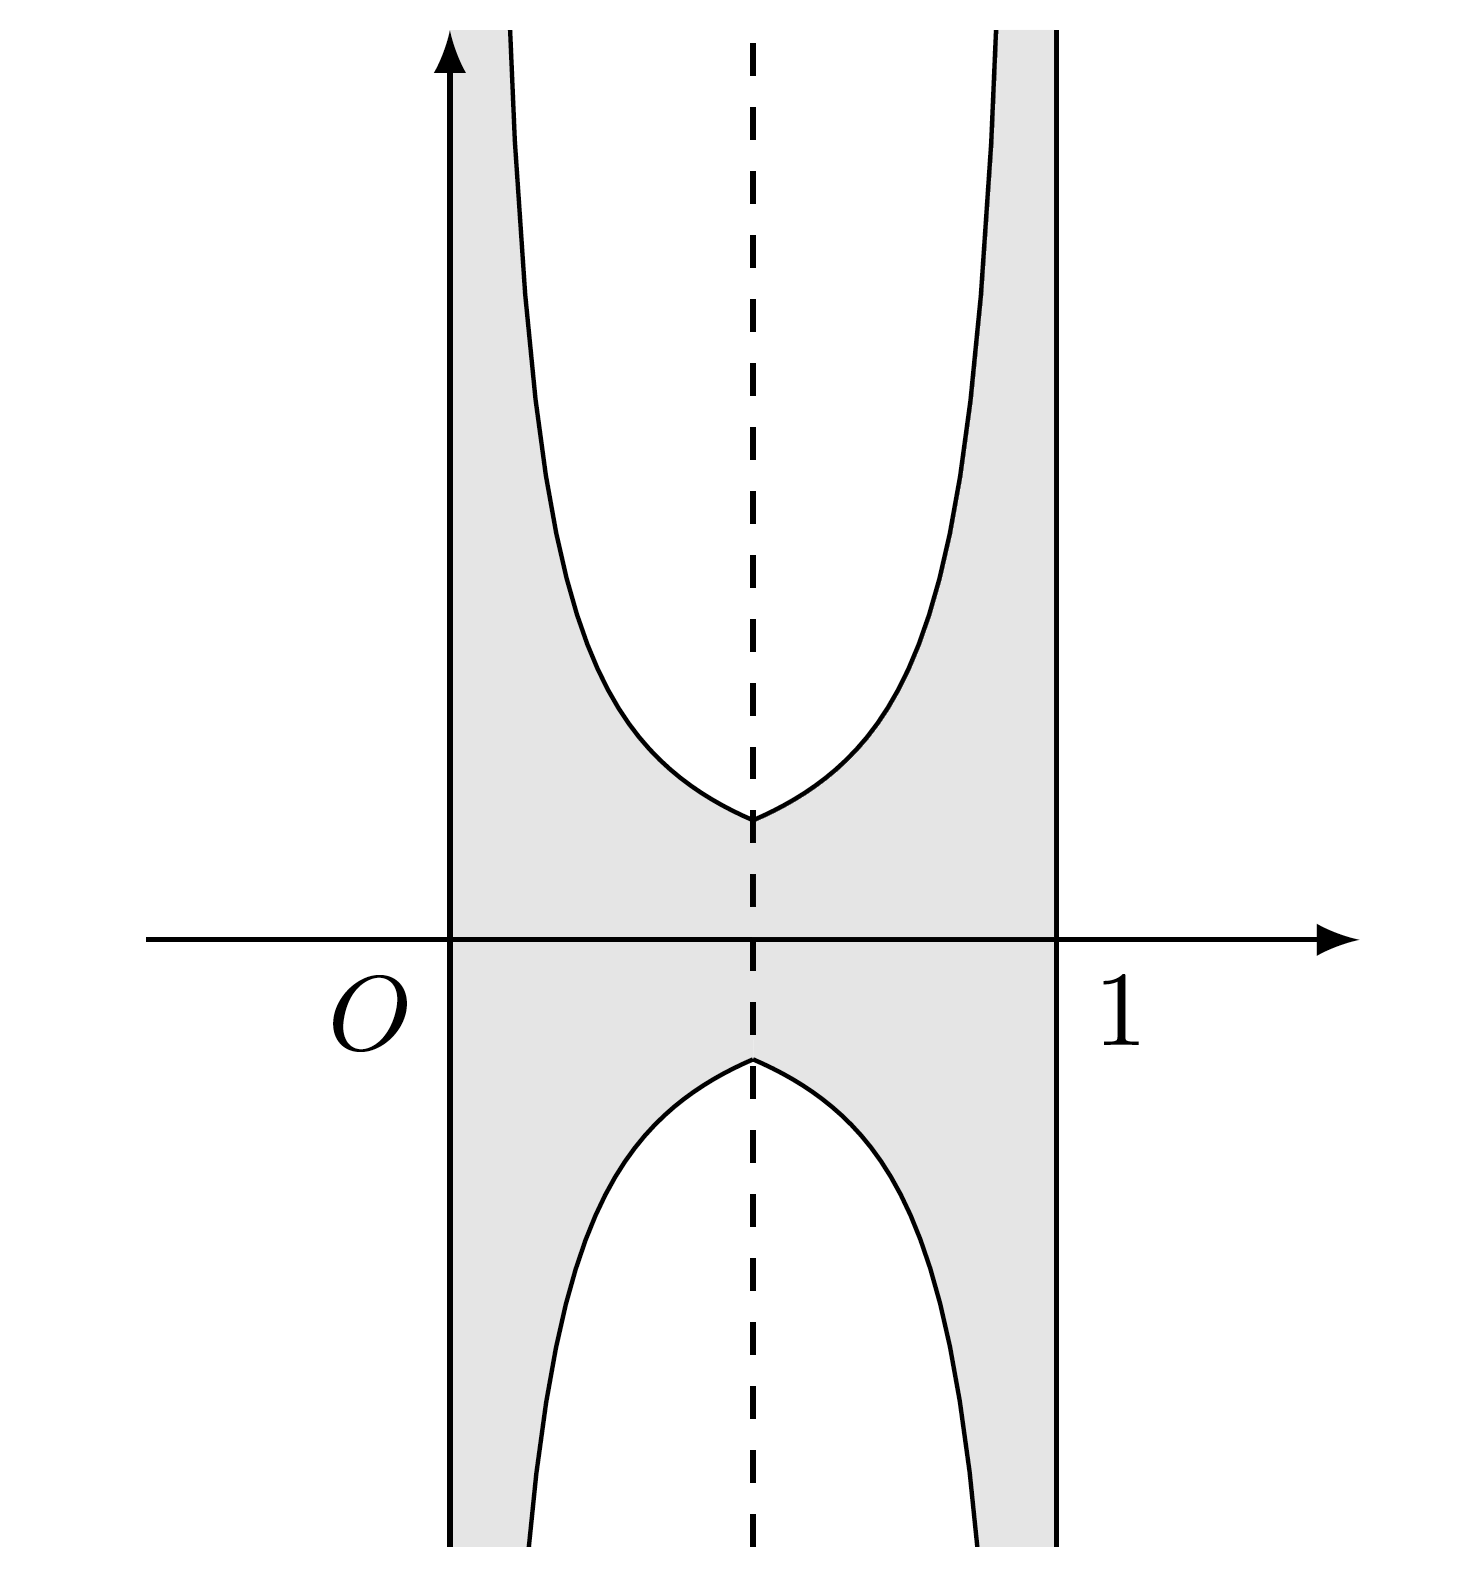
\includegraphics[width=0.5\textwidth]{fig_region_sans_zeros.png}
  \label{fig:region-sans-zero}
\end{figure}
    
\begin{proof} On a :
  \begin{itemize}
    \item $\forall c>0$,
    \item $\forall 0<\eta<\frac{c}{\ln|t|}$,
    \item $\forall s=\sigma+it\,\,\mathrm{avec}\,\,\sigma>1-\eta, |t|\geq2$,
  \end{itemize}
  alors on a bien $\sigma > 1-\frac{c}{\ln|t|}$, $|t|\geq2$, et on pose $s_0=1+\eta+it$. Par le corollaire \ref{cor:majoration-zeta-et-zeta-prime} sur les majorations de $\zeta$ et de $\zeta'$,

  \begin{align*}
    |\zeta(s)-\zeta(s_0)|
    = \left|\int_{s_0}^s\zeta'(\omega)\mathrm{d}\omega\right|
    &\leq C_0|s-s_0|\ln^2|t| \\
    &\leq 2C_0\eta\ln^2|t|,
  \end{align*}
  
  où l'intégrale est bien définie car $|t|\geq2$ donc on évite le pôle, et $C_0$ est une constante positive qui vient du $0$ de \ref{cor:majoration-zeta-et-zeta-prime}.

  On utilise maintenant l'inégalité fondamentale \ref{prop:zeta-inegalite-1} due à Mertens:
  \begin{align*}
    \zeta(s_0)
    &\geq \frac{1}{\zeta(1+\eta)^3|\zeta(1+\eta+2it)|} \\
    &\geq \frac{C_1\eta^3}{\ln|t|}
  \end{align*}

  où l'on a utilisé dans la deuxième inégalité la proposition \ref{cor:majoration-zeta-et-zeta-prime}, qui donne la constante positive $C_1$.
  \\

  D'où :
  \begin{align*}
    |\zeta(s)|
    &\geq |\zeta(s_0)| - |\zeta(s)-\zeta(s_0)| \\
    &\geq \frac{C_1^{1/4}\eta^{3/4}}{\ln^{1/4}|t|} - 2C_0\eta\ln^2|t|
  \end{align*}

  Choisissons alors $\eta$ pour que les deux termes se compensent, c'est-à-dire $\eta$ de l'ordre de $\ln^{-9}|t|$.
  \\

  Plus précisément, si l'on choisit :
  \[ \eta:=\frac{c}{\ln^9|t|}, \]

  Alors les hypothèses sont toujours vérifiées, on peut refaire le cheminement ci-dessus, et on a alors
  \[
    |\zeta(s)|
    \geq\frac{C_1^{1/4}c^{3/4}}{\ln^7|t|}-\frac{2C_0c}{\ln^7|t|}
    \geq\frac{C_2}{\ln^7|t|}.
  \]

  Donc $\zeta$ ne s'annule pas sur cette région, et la proposition est démontrée.
\end{proof}

Nous sommes maintenant en mesure de prouver le théorème des nombres premiers sous sa forme \ref{eq:tnp-erreur-1}. L'astuce est d'utiliser la formule de Perron, de briser le segment sur lequel s'effectue l'intégration, et de le remplacer par un contour qui contient le pôle $s=1$ (donc forcément débordant en partie sur le demi-plan $\sigma<1$). Le terme d'erreur vient alors de la valeur de l'intégrale sur les autres parties du contour. Formalisons cela.

\begin{proof}[Démonstration du théorème \ref{eq:tnp-erreur-1}]
  Nous avons vu à la proposition \ref{cor:zeta-sur-zeta-prime-o} 
  \[ \left|\frac{\zeta'(\sigma)}{\zeta(\sigma)}\right| = O_{\sigma\to1}\left(\frac{1}{\sigma-1}\right) \]
  Ainsi nous pouvons appliquer la seconde formule de Perron effective \ref{eq:perron-2-effective} avec :
  \begin{itemize}
    \item la série de Dirichlet $F(s)=\sum_{n\geq1}\frac{\Lambda(n)}{n^s}$
    \item $\alpha=1$, $\sigma_a=1$, et on a
      \[
        \sum_{n\geq1}\frac{\Lambda(n)}{n^{-\sigma}}
        = -\frac{\zeta'(\sigma)}{\zeta(\sigma)}
        = O((\sigma-1)^{-1})
        \]
    \item la fonction $B=\ln$ vérifie
    \[ \forall n\geq1,\quad\Lambda(n)\leq B(n) \]
  \end{itemize}
  On obtient, dans ce cas-là, pour $x\geq2$, $s=0$, $T\geq2$, et $\sigma_1=1+\frac{1}{\ln x}$ :
  \[ \psi(x) = \sum_{n\geq1}\Lambda(n) = \frac{1}{2\pi i}\int_{\sigma_1-iT}^{\sigma_1+iT}\left(-\frac{\zeta'(s)}{\zeta(s)}\right)\frac{x^s}{s}\mathrm{d}s\,+\,O\left(\frac{x\ln^2 x}{T}\right). \]
  Nous allons utiliser le théorème des résidus pour estimer l'intégrale, et choisir $T$ à la fin convenablement pour compenser les termes d'erreur.

  En fixant $c$ donné par le théorème \ref{eq:region-faible-sans-zero}, posons $\delta=\frac{c}{\ln^9T}$, $\sigma_0=1-\delta$, et rappelons que nous venons de poser $\sigma_1=1+\ln x$. Alors le rectangle $\mathbf{R}$ de sommets $(\sigma_0,\pm iT)$ et $(\sigma_1,\pm iT)$ est contenu dans cette région sans zéros (il déborde sur $\sigma\geq 1$, mais ce n'est pas grave car $\zeta$ n'a pas de zéros non plus sur cette région). En notant $f(s)=\left(-\frac{\zeta'(s)}{\zeta(s)}\right)\frac{x^s}{s}$ l'intégrande, on a alors que $s=1$ est l'unique pôle de $f$ dans ce rectangle $\mathbf{R}$. Le théorème des résidus nous fournit alors (le terme à l'intérieur de l'intégrale, $f(s)\mathrm{d}s$, est omis pour clarté) :
  \[ \psi(x) = \mathrm{Res}(f,1) + \frac{1}{2\pi i}\left(
    \int_{\sigma_0-iT}^{\sigma_0+iT}
    +\int_{\sigma_0+iT}^{\sigma_1+iT}
    -\int_{\sigma_0-iT}^{\sigma_1-iT}
    \right)
    +O\left(\frac{x\ln^2x}{T}\right). \]

  \begin{figure}[h]
    \centering
    \caption{Répresentation du contour.}
    \begin{picture}(300,300)
      \put(0,0){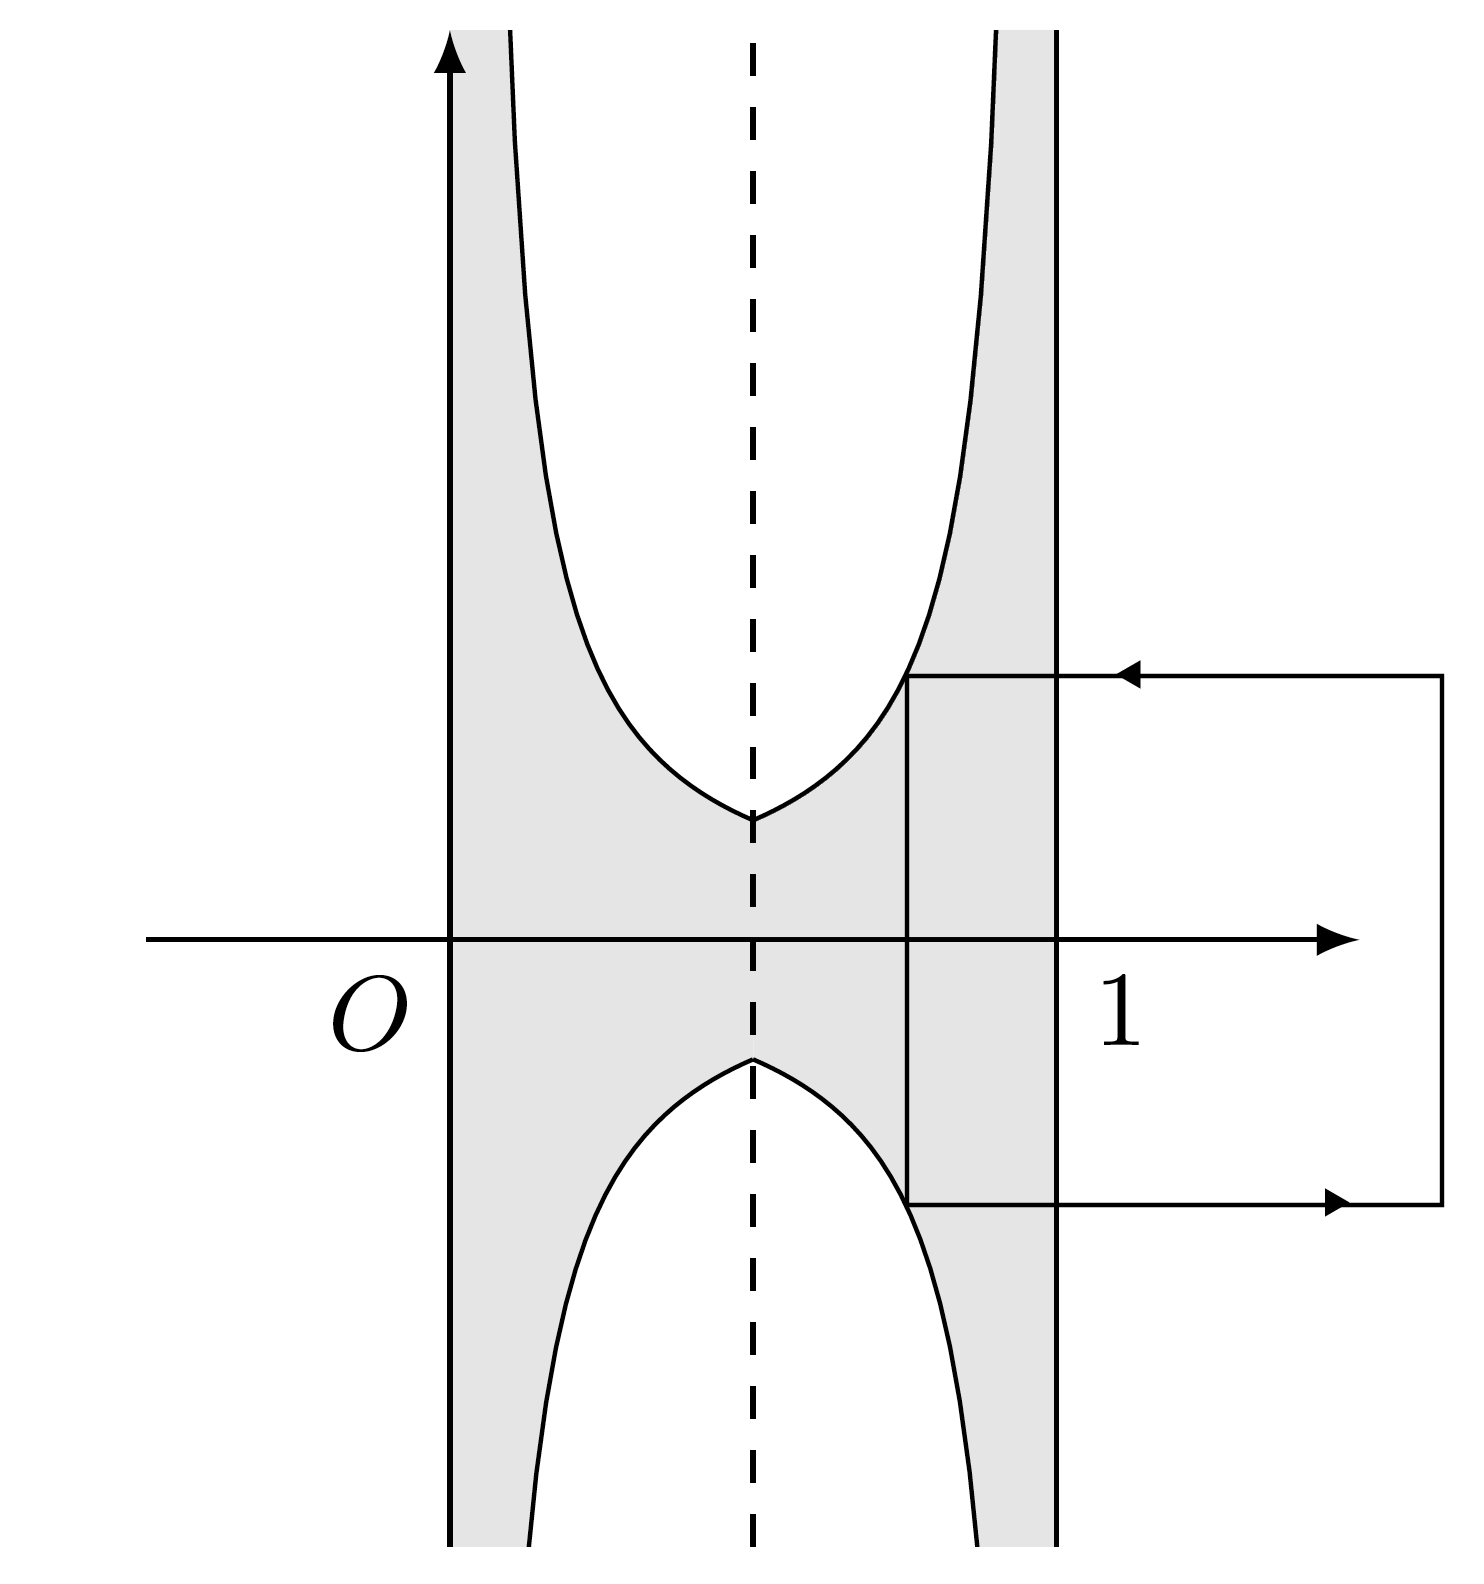
\includegraphics[width=0.8\textwidth]{fig_contour.png}}
      \put(50,50){hello}
      \put(220,60){$\mathbf{R}$}
      \put(150,175){$\sigma_0+iT$}
      \put(150,60){$\sigma_0-iT$}
      \put(255,175){$\sigma_1+iT$}
      \put(255,60){$\sigma_1-iT$}
    \end{picture}
    \label{fig:contour-affaiblie}
  \end{figure}

  Nous pouvons facilement vérifier que $\mathrm{Res}(f,1)=x$, car $\zeta$ a un pôle simple en $s=1$, donc
  \begin{equation}\label{eq:tnp-faible-3-integrales}
    \psi(x) = x +\frac{1}{2\pi i}\left(
      \int_{\sigma_0-iT}^{\sigma_0+iT}
      +\int_{\sigma_0+iT}^{\sigma_1+iT}
      -\int_{\sigma_0-iT}^{\sigma_1-iT}
    \right)
    +O\left(\frac{x\ln^2x}{T}\right)
  \end{equation}

  On voit déjà le terme $x$ de l'énoncé apparaître, essayons donc d'estimer les trois intégrales.
  
  \textbf{Estimation de la 2ème intégrale}. Commençons par celle du milieu, qui a lieu sur le petit segment horizontal du haut. Notons $I_h$ ce segment, et on a la majoration grossière :
  \begin{align*}
    |f(s)| = \left|\left(-\frac{\zeta'(s)}{\zeta(s)}\right)\frac{x^s}{s}\right| & \leq\frac{x^{\sigma_1}}{T}\max_{I_h}|\zeta'|\max_{I_h}\left|\frac{1}{\zeta}\right| \\
    & \leq\frac{x}{T}\max_{I_h}|\zeta'|\max_{I_h}\left|\frac{1}{\zeta}\right|.
  \end{align*}
  (Astuce : l'inégalité $|s|\geq T$ se voit mieux géométriquement.)

  Mais on a déjà vu :
  \begin{itemize}
    \item $\max|\zeta'| = O(\ln^2 T)$ dans la proposition \ref{cor:majoration-zeta-et-zeta-prime},
    \item $\max|\frac{1}{\zeta}| = O(\ln^7 T)$ dans le théorème juste au-dessus \ref{eq:region-faible-sans-zero}.
  \end{itemize}

  Et donc
  \[ |f(s)| = O\left(\frac{x}{T}\ln^9T\right) \]

  Comme la longueur du segement est $\sigma_1-\sigma_0=1/\ln x+\delta=O(1)$, on a que
  \begin{equation}\label{eq:tnp-faible-3-integrales-part1}
    \int_{\sigma_0+iT}^{\sigma_1+iT}f(s)\mathrm{d}s = O\left(\frac{x}{T}\ln^9T\right)
  \end{equation}

  \textbf{Estimation de la 3ème intégrale}. Par symétrie par rapport à l'axe des abscisses, la troisième intégrale sur le segment de bas $I_b$ dans \ref{eq:tnp-faible-3-integrales} est également $O\left(\frac{x}{T}\ln^9T\right)$.
  \\

  \textbf{Estimation de la 1ère intégrale}. Reste à évaluer la première intégrale sur le segment vertical de gauche $I_g$. Pareil, majorons grossièrement :
  \begin{align*}
    |f(s)| = \left|\left(-\frac{\zeta'(s)}{\zeta(s)}\right)\frac{x^s}{s}\right| & \leq\frac{x^{\sigma_0}}{|s|}\max_{I_g}|\zeta'|\max_{I_g}\left|\frac{1}{\zeta}\right| \\
    & = O\left(\frac{x^{\sigma_0}}{|s|}\max_{I_g}|\zeta'|\ln^7 T\right)
  \end{align*}

  On est tenté ici d'utiliser encore une fois la proposition \ref{cor:majoration-zeta-et-zeta-prime} pour majorer $|\zeta'|$. Mais il faut faire attention, car on n'a plus le $|t|\geq2$ nécessaire pour \ref{cor:majoration-zeta-et-zeta-prime}, car ce segment est assez proche du pôle $s=1$, donc $\max_{I_g}|\zeta'|$ peut devenir assez importante. Mais par hypothèse, $\frac{1}{|\sigma-1|}=O(\ln^9|t|)$ Nous utilisons la proposition \ref{prop:majorations-pres-du-pole} pour avoir la majoration
  % https://web.stanford.edu/~tonyfeng/riemann_zeta.pdf
  \begin{equation}\label{eq:tnp-faible-3-integrales-part2}
    \max_{I_g}|\zeta'|=O(\ln^{18}T)
  \end{equation}


  \textbf{Conclusion}. En combinant \ref{eq:tnp-faible-3-integrales-part1} et \ref{eq:tnp-faible-3-integrales-part2} et en les injectant dans \ref{eq:tnp-faible-3-integrales}, on obtient
  \[ \psi(x) = x
  + O\left(x^{\sigma_0}\ln^{25}x\int_{-T}^T\frac{1}{1+|t|}\mathrm{d}t\right)
  + O\left(\frac{x}{T}\ln^9T\right)
  + O\left(\frac{x\ln^2x}{T}\right)
  \]

  L'intégrale est $O(\ln T)$, et le dernier terme peut être absorbé dans $O\left(\frac{x}{T}\ln^9T\right)$, donc
  \[ \psi(x) = x + O(x^{\sigma_0}\ln^{26}x) + O\left(\frac{x}{T}\ln^9T\right) \]

  En majorant encore plus grossièrement, c'est-à-dire $O(\ln^9 T) = O(\ln^{26} T)$, on peut factoriser
  \begin{align*}
    \psi(x) &= x + O\left(x\ln^{26} x\left(x^{-\delta}+\frac{1}{T}\right)\right) \\
    &= x + O\left(x\ln^{26} x\left(\mathrm{e}^{-\frac{c\ln x}{\ln^9 T}}+\mathrm{e}^{-\ln T}\right)\right)
  \end{align*}

  Il faut noter que les deux termes en exponentiel varient en sens opposés lorsque $T$ augmente. On peut les rendre égaux en choisissant $T=\exp(\ln^{1/10}x)$, auquel cas on a :
  \[
    \psi(x) = x + O(x\ln^{26} x\mathrm{e}^{-c\ln^{1/10}x}).
  \]

  Il suffit d'essayer d'enlever le terme en $\ln^{26} x$, un choisissant un $c$ plus petit. Ceci est possible du fait que $\ln\ln x = o(\ln^\alpha x)$, pour tout $\alpha>0$. En particulier, pour $x$ assez grand, $\ln\ln x < \frac{1}{30}\ln^{1/10} x$, et donc $\ln x < \mathrm{e}^{\frac{c}{30}\ln^{1/10}x}$, puis $\ln^{26} x < \mathrm{e}^{(c-\frac{2}{15}c)\ln^{1/10}x}$.
  \\

  En posant $c'=\frac{2}{15}c$, on obtient :
  \[ \psi(x) = x + O(x\mathrm{e}^{-c'\ln^{1/10}x}). \]
\end{proof}

%%%%%%%%%%%%%%%%%%%%%%%%%%%%%%%%%%%%%%%%%%%%%%%%%%%%%%%%%%%%%%%%%%%%%%%%%%%%%%%%
%%%%%%%%%%%%%%%%%%%%%%%%%%%%%%%%%%%%%%%%%%%%%%%%%%%%%%%%%%%%%%%%%%%%%%%%%%%%%%%%
\section{Région classique sans zéros}\label{section:region-classique}
%%%%%%%%%%%%%%%%%%%%%%%%%%%%%%%%%%%%%%%%%%%%%%%%%%%%%%%%%%%%%%%%%%%%%%%%%%%%%%%%
%%%%%%%%%%%%%%%%%%%%%%%%%%%%%%%%%%%%%%%%%%%%%%%%%%%%%%%%%%%%%%%%%%%%%%%%%%%%%%%%

Le terme d'erreur $O(x\mathrm{e}^{-c\ln^{1/10}x})$ dans \ref{eq:tnp-erreur-1} n'est pas terrible, on peut peut-être l'améliorer. En diagnostiquant la preuve ci-dessus, on remarque que ce terme d'erreur vient en très grande partie de l'intégrale sur le segment vertical de gauche. En fait, plus on arrive à décaler ce segment vers la gauche, plus l'intégrale sera petite.

Mais pour ce faire, il nous faut trouver une région sans zéros plus grande que celle du théorème \ref{eq:region-faible-sans-zero}. Le but de cette section est donc de démontrer le théorème suivante :

\begin{theorem}[Région classique sans zéro]\label{thm:region-classique-sans-zero}
  Il existe un réel $c>0$ tel que la fonction $\zeta$ ne s'annule pas sur la région du plan définie par
  \[ |t|\geq2 \quad \mathrm{et} \quad \sigma\geq1-\frac{c}{\ln|t|} \]
\end{theorem}

La preuve de la région affaiblie dans la section précédente était assez simple et ne requérait pas d'outils très avancés. Mais nous allons voir que cette preuve ci-dessus utilise des outils tels que le produit de Hadamard ou l'analyse de la fonction $\Gamma$.

\begin{proof}
  Soit $\rho_0=\beta+i\gamma$ un zéro non-trivial de $\zeta$, avec $|\gamma|\geq2$. Nous allons montrer qu'il existe un $c>0$, indépendent de $\rho_0$, tel que 
  \[ \beta<1-\frac{c}{\ln|\gamma|}. \]

  Nous partons de la propositions \ref{cor:zeta-zeta-prime-van-mangoldt}, qui nous fournit la série de Dirichlet à termes positifs ou nuls :
  \[ -\frac{\zeta'(s)}{\zeta(s)} = \sum_{n\geq1}\frac{\Lambda(n)}{n^s}. \]

  Son abscisse de convergence est $1$, et on a d'après la formule \ref{thm:mertens-positif} due à Mertens, $\forall\sigma>1, \forall t\in\mathbb{R}$

 \begin{equation}\label{eq:mertens-zeta-zeta-prime}
  - 3\frac{\zeta'(\sigma)}{\zeta(\sigma)}
  - 4\Re\frac{\zeta'(\sigma+it)}{\zeta(\sigma+it)}
  - \Re\frac{\zeta'(\sigma+2it)}{\zeta(\sigma+2it)}
  \geq0.
 \end{equation}

  Nous allons majorer les 3 termes ci-dessus.
  \\

  \textbf{1er terme}. Il suffit d'utiliser le fait que 1 est un pôle d'ordre 1 et de résidu 1 pour $\zeta$, démontré dans la  proposition \ref{prop:zeta-sur-zeta-prime-1-sur-holomorphe},
  \[ -3\frac{\zeta'(\sigma)}{\zeta(\sigma)} \leq \frac{3}{\sigma-1} + O(1). \]

  \textbf{2ème terme}. En dérivant logarithmitiquement la formule du produit de Hadamard \ref{thm:produit-hadamard} de $\zeta$, on a, pour $s\neq1$ et $s\neq\rho$:

  \begin{align}
    -\frac{\zeta'(s)}{\zeta(s)}
    &= -b + \frac{1}{s-1}
    + \frac{\Gamma'(\frac{s}{2}+1)}{2\Gamma(\frac{s}{2}+1)}
    - \sum_{\rho}\left(\frac{-1}{1-\frac{s}{\rho}} + \frac{1}{\rho}\right) \\
    &= -b + \frac{1}{s-1}
    + \frac{\Gamma'(\frac{s}{2}+1)}{2\Gamma(\frac{s}{2}+1)}
    - \sum_{\rho}\left(\frac{1}{\rho} + \frac{1}{s-\rho} \right). \label{eq:hadamard-derivee-logarithmique}
  \end{align}

  Clairement, les deux premiers termes sont majorés en norme au voisinage de $+\infty$ :
  \[ -b + \frac{1}{s-1} = O(1) \]

  On a également, en utlisant la formule de Stirling complexe \ref{cor:gamma-gamma-prime-majoration}, on a
  \[ -\Re\frac{\zeta'(s)}{\zeta(s)} = O(\ln(|t|))\quad(\sigma>1, |t|\geq2). \]

  On a donc temporairement

  \begin{equation}\label{eq:thm-region-classique-temporaire}
    - \Re\frac{\zeta'(s)}{\zeta(s)}
    \leq O(1)
    + O(\ln|t|)
    - \sum_{\rho}\Re\left(\frac{1}{\rho} + \frac{1}{s-\rho} \right).
  \end{equation}

  Par ailleurs, remarquons que dans la somme, chaque terme est strictement positif. Nous utilisons le fait que tous ces $\rho$ zéros non-triviaux de $\zeta$ sont situés dans la bande critique $0<t<1$ (lire la section \ref{section:localisation-zeros}). On a que tous les $\rho$ vérifient $\Re\rho>0$, donc $\Re\frac{1}{\rho}>0$. De même $\Re s=\sigma>1$ et $\Re\rho<1$, donc $\Re(s-\rho)>0$, donc $\Re\frac{1}{s-\rho}>0$. 
  \\

  Fixons un complexe $s=\sigma+i\gamma$ avec $\sigma>1$ et de partie imaginaire identique à $\rho_0$. On applique alors l'équation \ref{eq:thm-region-classique-temporaire} à $s$. Les termes de la sommes étant positifs, on ne garde qu'un seul, celui qui correspond à $\frac{1}{s-\rho_0}=\frac{1}{\sigma-\beta}$.
  \begin{align*}
    - \Re\frac{\zeta'(\sigma+i\gamma)}{\zeta(\sigma+i\gamma)}
    &\leq O(\ln|t|)
    -\frac{1}{\sigma-\beta} \\
    &\leq\frac{c'}{2}\ln|\gamma|
    -\frac{1}{\sigma-\beta}
  \end{align*}
  pour une certain constante $c'>0$, ne dépendant ni de $s$ ni de $\rho_0$.
  \\

  \textbf{3ème terme}. On applique le même raisonnement que pour le 2ème terme à $s=\sigma+2i\gamma$, et on ne garde aucun terme dans la somme \ref{eq:thm-region-classique-temporaire} (possible, car les termes sont tous strictement positifs).
  En choisissant $c'$ assez grand, on peut alors trouver que pour la même constante $c'$, on a
  \[
    - \Re\frac{\zeta'(\sigma+2i\gamma)}{\zeta(\sigma+2i\gamma)}
    \leq\frac{c'}{2}\ln|\gamma|
  \]

  \textbf{Conclusion}. En reportant les 3 majorations dans l'inégalité \ref{eq:mertens-zeta-zeta-prime}, on obtient
  \[
    \frac{-3}{\sigma-1}+\frac{4}{\sigma-\beta}-c'\ln|\gamma|\leq0.
  \]

  On isole $1-\beta$. Comme la constante $c'$ ne dépend pas du $\rho_0$ initialement choisi, on a donc, pour tout $\sigma>1$, pour tout zéro non-trivial $\rho=\beta+i\gamma$ tel que $|\gamma|\geq2$,
  \begin{align*}
    1-\beta
    &\geq \frac{4}{c'\ln|\gamma|+\frac{3}{\sigma-1}} - (\sigma -1) \\
    &=\frac{1/2}{7c'\ln|\gamma|} \\
    &=\frac{c}{\ln|\gamma|}
  \end{align*}
  où l'on a posé $c=c'/14>0$. Ceci achève la démonstration.
\end{proof}

%%%%%%%%%%%%%%%%%%%%%%%%%%%%%%%%%%%%%%%%%%%%%%%%%%%%%%%%%%%%%%%%%%%%%%%%%%%%%%%%
\subsection{Majorations dans cette région}
%%%%%%%%%%%%%%%%%%%%%%%%%%%%%%%%%%%%%%%%%%%%%%%%%%%%%%%%%%%%%%%%%%%%%%%%%%%%%%%%

Pour prouver le théorème des nombres premiers en utilisant cette région sans zéros, nous avons besoin de quelques majorations.

\begin{proposition}\label{prop:majoration-zeta-zeta-prime-region-classique}
  Il existe une constante positive $c$ telle que l'on ait, pour $|t|\geq2$ et $\sigma\geq1-\frac{c}{\ln|t|}$,
  \[ \frac{\zeta'(s)}{\zeta(s)} = O(\ln|t|) \]
\end{proposition}

\begin{proof}
  D'après le théorème précédent \ref{thm:region-classique-sans-zero}, on peut fixer un $c$, que l'on peut supposer inférieur à $\frac{1}{16}$, tel que l'on ait pour tout $\rho=\beta+i\gamma$ zéro non trivial de $\zeta$, $\beta<1-\frac{8c}{\ln|\gamma|}$. Soit maintenant $s=\sigma+it$ un nombre complexe tel que $|t|\geq 4$ et $\sigma>1-\frac{4c}{\ln |t|}$. On pose :
  \[
    \mu=\inf_\rho\left\{\Re\left(\frac{1}{\rho}+\frac{1}{s-\rho}\right)\right\}
  \]

  \textbf{1ère étape} : $\mu\geq0$. On fixe un $\rho$ zéro non trivial de $\zeta$, et on fait une distinction de cas.

  \textit{1er cas}: $|s-\rho|>\frac{1}{2}|\rho|$. On peut calculer :
  \begin{align}
    \Re\left(\frac{1}{\rho}+\frac{1}{s-\rho}\right)
    &= \frac{\beta}{|\rho|^2} + \frac{\sigma - \beta}{|s-\rho|^2} \\
    &= \frac{\beta|s-\rho|^2 + |\rho|^2(\sigma-\beta)}{|\rho|^2|s-\rho|^2} \\
    &= \frac{\frac{\theta^2 \beta}{4} + \sigma - \beta}{|s-\rho|^2} \label{eq:re-rho-s-moins-rho}
  \end{align}

  où l'on a posé $\theta = 2\frac{|s-\rho|}{|\rho|}$. Par hypothèse de notre 1er cas, $\theta>1$. 
    
  \begin{align*}
    \Re\left(\frac{1}{\rho}+\frac{1}{s-\rho}\right)
    & > \frac{\frac{\beta}{4} + \sigma - \beta}{|s-\rho|^2} \\
    & = \frac{\sigma - \frac{3}{4}\beta}{|s-\rho|^2} \\
    & > \frac{\sigma - \frac{3}{4}}{|s-\rho|^2}
  \end{align*}

  où on a utlisé dans la dernière inégalité $\beta<1$, car $\rho$ est dans la bande critique. Comme on a pris $|t|\geq 4$ et $c<\frac{1}{16}$, on a $\sigma\geq 1-\frac{1}{4\ln 4}\approx 0.81$, donc $\sigma-0.75>0$, donc $ \Re\left(\frac{1}{\rho}+\frac{1}{s-\rho}\right)>0$. Et il suit que $\mu\geq0$.
  \\

  \textit{2ème cas}: $|s-\rho|\leq\frac{1}{2}\rho$. Alors en remplaçant $s$ et $\rho$ par leurs parties réelles et imaginaires, 
  \begin{align*}
    4((\sigma-\beta)^2 + (t-\gamma)^2)
    &\leq \gamma^2 + \beta^2 \\
    &< \gamma^2 + 1 \\
    &\leq (|\gamma|+1)^2
  \end{align*}

  en utilisant le fait que $\beta<1$ dans la deuxième inégalité. En minorant $(\sigma-\beta)^2\geq 0$, on a alors $4(t-\gamma)^2\leq (|\gamma|+1)^2$, donc $2|t-\gamma| \leq |\gamma| + 1$. Par ailleurs, par inégalité triangulaire, on a aussi $2|t-\gamma| \geq 2||t| - |\gamma||$. On va montrer par (encore une !) distinction de cas que cela implique toujours :
  \[
    |\gamma|\leq 2t+1.
  \]

  \begin{itemize}
    \item si $|\gamma|\geq t$, alors $|\gamma|+1\geq 2|\gamma|-2t$, soit $|\gamma|\leq 2t+1$.
    \item si $|\gamma|\leq t$, alors l'inégalité annoncée est triviale.
  \end{itemize}

  Maintenant que l'on a établi $|\gamma|\leq 2t+1$, l'inégalité $\beta< 1-\frac{8c}{\ln|\gamma|}$ devient :
  \[
    \beta
    < 1-\frac{8c}{\ln(2t+1)}
    \leq 1-\frac{4c}{\ln t}
    \leq \sigma
  \]

  où la deuxième égalité vient de l'étude de la fonction $t\mapsto\frac{8c}{\ln(2t+1)}-\frac{4c}{\ln t}$, qui est positive ou nulle pour $t\geq 1+\sqrt{2}$, ce qui est bien notre case puisque l'on a pris $t\geq 4\geq 1+\sqrt{2}$. On réécrit l'équation \ref{eq:re-rho-s-moins-rho}, toujours valable :
  \[
    \Re\left(\frac{1}{\rho}+\frac{1}{s-\rho}\right)
    = \frac{\frac{\theta^2 \beta}{4} + \sigma - \beta}{|s-\rho|^2}.
  \]

  Mais on vient de montrer que $\beta<\sigma$, donc cette partie réelle est strictement positive. Par passage à la borne inférieure, $\mu\geq 0$.
  \\

  \textbf{2ème étape}. On part de la formule de dérivée logarithmique du produit de Hadamard, donnée en \ref{eq:hadamard-derivee-logarithmique} dans le théorème \ref{thm:region-classique-sans-zero}. En prenant la partie réelle de cette formule, les parties réelles des termes de la somme étant tous positifs ou nuls d'après la première étape, on a
  \[
    \Re\left(-\frac{\zeta'(s)}{\zeta(s)}\right)
    \leq \Re\left(-b + \frac{1}{s-1}\right)
    + \Re\left(\frac{\Gamma'(\frac{s}{2}+1)}{2\Gamma(\frac{s}{2}+1)}\right).
  \]

  Notons que dans la démonstration du théorème \ref{thm:region-classique-sans-zero}, les parties réelles des termes de la somme étaient aussi positives, mais celà découlait du fait que $s$ était de partie réelle strictement supérieure à 1. Nous avons ici un $\Re(s)<1$, d'où la nécessité de la 1ère étape.
  \\

  En utilisant encore une fois la formule de Stirling complexe (corollaire \ref{cor:gamma-gamma-prime-majoration}), on obtient un $K>0$ tel qu'au voisinage de $+\infty$
  \begin{equation}\label{eq:reel-zeta-zeta-prime-k-lnt}
    \Re\left(-\frac{\zeta'(s)}{\zeta(s)}\right) \leq K\ln t.
  \end{equation}

  Posons désormais quelques variables :
  \begin{itemize}
    \item $s=\sigma+it$ quelconque, avec $t\geq 5$ et $\sigma\geq1-\frac{c}{\ln t}$,
    \item $\eta=\frac{c}{\ln t}$,
    \item $s_0 = 1 + \eta + it$,
    \item $\omega$ dans le disque $|\omega|\leq 4\eta$,
    \item $(\sigma',\,t')$ tel que $s_0+\omega=\sigma'+it'$.
  \end{itemize}
  
  Alors comme $\eta\geq\frac{1}{16\ln 5}\approx 0.04$, on a $4\eta\leq 1$, donc $t'=t+\Im(\omega)\geq 4$. De même, $\sigma'=1+\eta+\Re(\omega)\geq 1+5\eta\geq1-\frac{4c}{\ln t'}$.
  \\
  Ainsi $s_0+\omega$ satisfait aux hypothèses qui conduisent à l'équation \ref{eq:reel-zeta-zeta-prime-k-lnt} et on peut écrire :
  \begin{align*}
    \Re\left(-\frac{\zeta'(s_0+\omega)}{\zeta(s_0+\omega)}\right)
    &\leq K\ln t' \\
    &\leq K\ln (t+4\eta) \\
    &\leq K\ln (2t) \\
    &\leq 2K\ln (t)
  \end{align*}

  où la dernière inégalité vient de $2X\leq X^2$ pour $X\geq 2$ (en étudiant rapidement le polynôme $X(X-2)$), ainsi que de la croissance de $\ln$.
  \\

  \textbf{Conclusion}. On a majoré la partie réelle, et on veut majorer le module : on cherche donc à appliquer le théorème de Borel-Carathéodory \ref{lem:borel-caratheodory}. Posons donc
  \[
    \forall|\omega|\leq 4\eta,\quad
    F(\omega)=\frac{\zeta'(s_0)}{\zeta(s_0)}-\frac{\zeta'(s_0+\omega)}{\zeta(s_0+\omega)}.
  \]

  Alors $F$ est holomorphe sur le disque de centre 0 et de rayon $4\eta$, $F(0)=0$, et l'inégalité trouvée en fin de deuxième étape montre que $\Re(F)$ est majorée par $A=2K\ln t+\left|\frac{\zeta'(s_0)}{\zeta(s_0)}\right|$. Ce lemme nous dit donc :
  \[
    \forall |\omega|<4\eta,\quad
    \left|\frac{\zeta'(s_0)}{\zeta(s_0)}-\frac{\zeta'(s_0+\omega)}{\zeta(s_0+\omega)}\right|
    \leq\frac{4K\ln t|\omega|}{4\eta-|\omega|}.
  \]

  Or, on a $s-s_0=1+\eta-\sigma\geq 2\eta$, donc on peut appliquer cette majoration en $\omega=s-s_0$ et majorer $|s-s_0|\geq 2\eta$ :
  \[
    \left|\frac{\zeta'(s_0)}{\zeta(s_0)}-\frac{\zeta'(s)}{\zeta(s)}\right|
    \leq 4K\ln t.
  \]

  Puis, par inégalité triangulaire,
  \[
    \left|\left|\frac{\zeta'(s_0)}{\zeta(s_0)}\right|-\left|\frac{\zeta'(s)}{\zeta(s)}\right|\right|
    \leq 4K\ln t,
  \]

  ce qui implique :
  \begin{equation}\label{eq:zeta-zeta-prime-4k}
    \left|\frac{\zeta'(s)}{\zeta(s)}\right|
    \leq 4K\ln t
    + \left|\frac{\zeta'(s_0)}{\zeta(s_0)}\right|.
  \end{equation}

  Mais en prenant l'écriture de $\zeta'/\zeta$ avec la fonction de van Mangoldt (proposition \ref{cor:zeta-zeta-prime-van-mangoldt}),
  \[
    \left|\frac{\zeta'(s_0)}{\zeta(s_0)}\right|
    \leq \sum_{n=1}^{+\infty}\frac{\Lambda(n)}{n^{1+\eta}}
    = \frac{\zeta'(1+\eta)}{\zeta(1+\eta)}.
  \]

  Le pôle en 1 de $\zeta'/\zeta$ est simple et de résidu -1 (proposition \ref{prop:zeta-sur-zeta-prime-1-sur-holomorphe}), donc au voisinage de 1,
  \[
    \frac{\zeta'(1+\eta)}{\zeta(1+\eta)}
    =\frac{1}{\eta} + O(1).
  \]

  Finalement, en remplaçant dans $\ref{eq:zeta-zeta-prime-4k}$,
  \[
    \left|\frac{\zeta'(s)}{\zeta(s)}\right| = O(\ln t).
  \]
\end{proof}

%%%%%%%%%%%%%%%%%%%%%%%%%%%%%%%%%%%%%%%%%%%%%%%%%%%%%%%%%%%%%%%%%%%%%%%%%%%%%%%%
\subsection{Théorème des nombres premiers}
%%%%%%%%%%%%%%%%%%%%%%%%%%%%%%%%%%%%%%%%%%%%%%%%%%%%%%%%%%%%%%%%%%%%%%%%%%%%%%%%

\begin{theorem}[Théorème des nombres premiers avec terme d'erreur, de la Vallée Poussin, 1899]\label{thm:tnp-terme-erreur-classique}
  Il existe une constante réelle $c>0$ telle que l'on ait, au voisinage de $+\infty$,
  \begin{equation}
    \psi(x)=x+O(x\mathrm{e}^{-c\sqrt{\ln x}})
  \end{equation}
\end{theorem}

\begin{proof}
  La preuve est exactement la même que celle du théorème \ref{eq:tnp-erreur-1}, sauf qu'on utilise la nouvelle région sans zéros que l'on vient de définir plus haut, et le rectangle est de sommets $(\sigma_0,\pm iT)$, $(\sigma_1,\pm iT)$, avec 
  \begin{itemize}
    \item $\sigma_0=1-\frac{c}{\ln(T)}$
    \item $\sigma_1=1+1/\ln x$
  \end{itemize}

  \begin{figure}[h]
    \centering
    \caption{Répresentation du contour. C'est la même figure que \ref{fig:contour-affaiblie}, mais il faut imaginer que la partie grise ici est plus grande.}
    \begin{picture}(300,300)
      \put(0,0){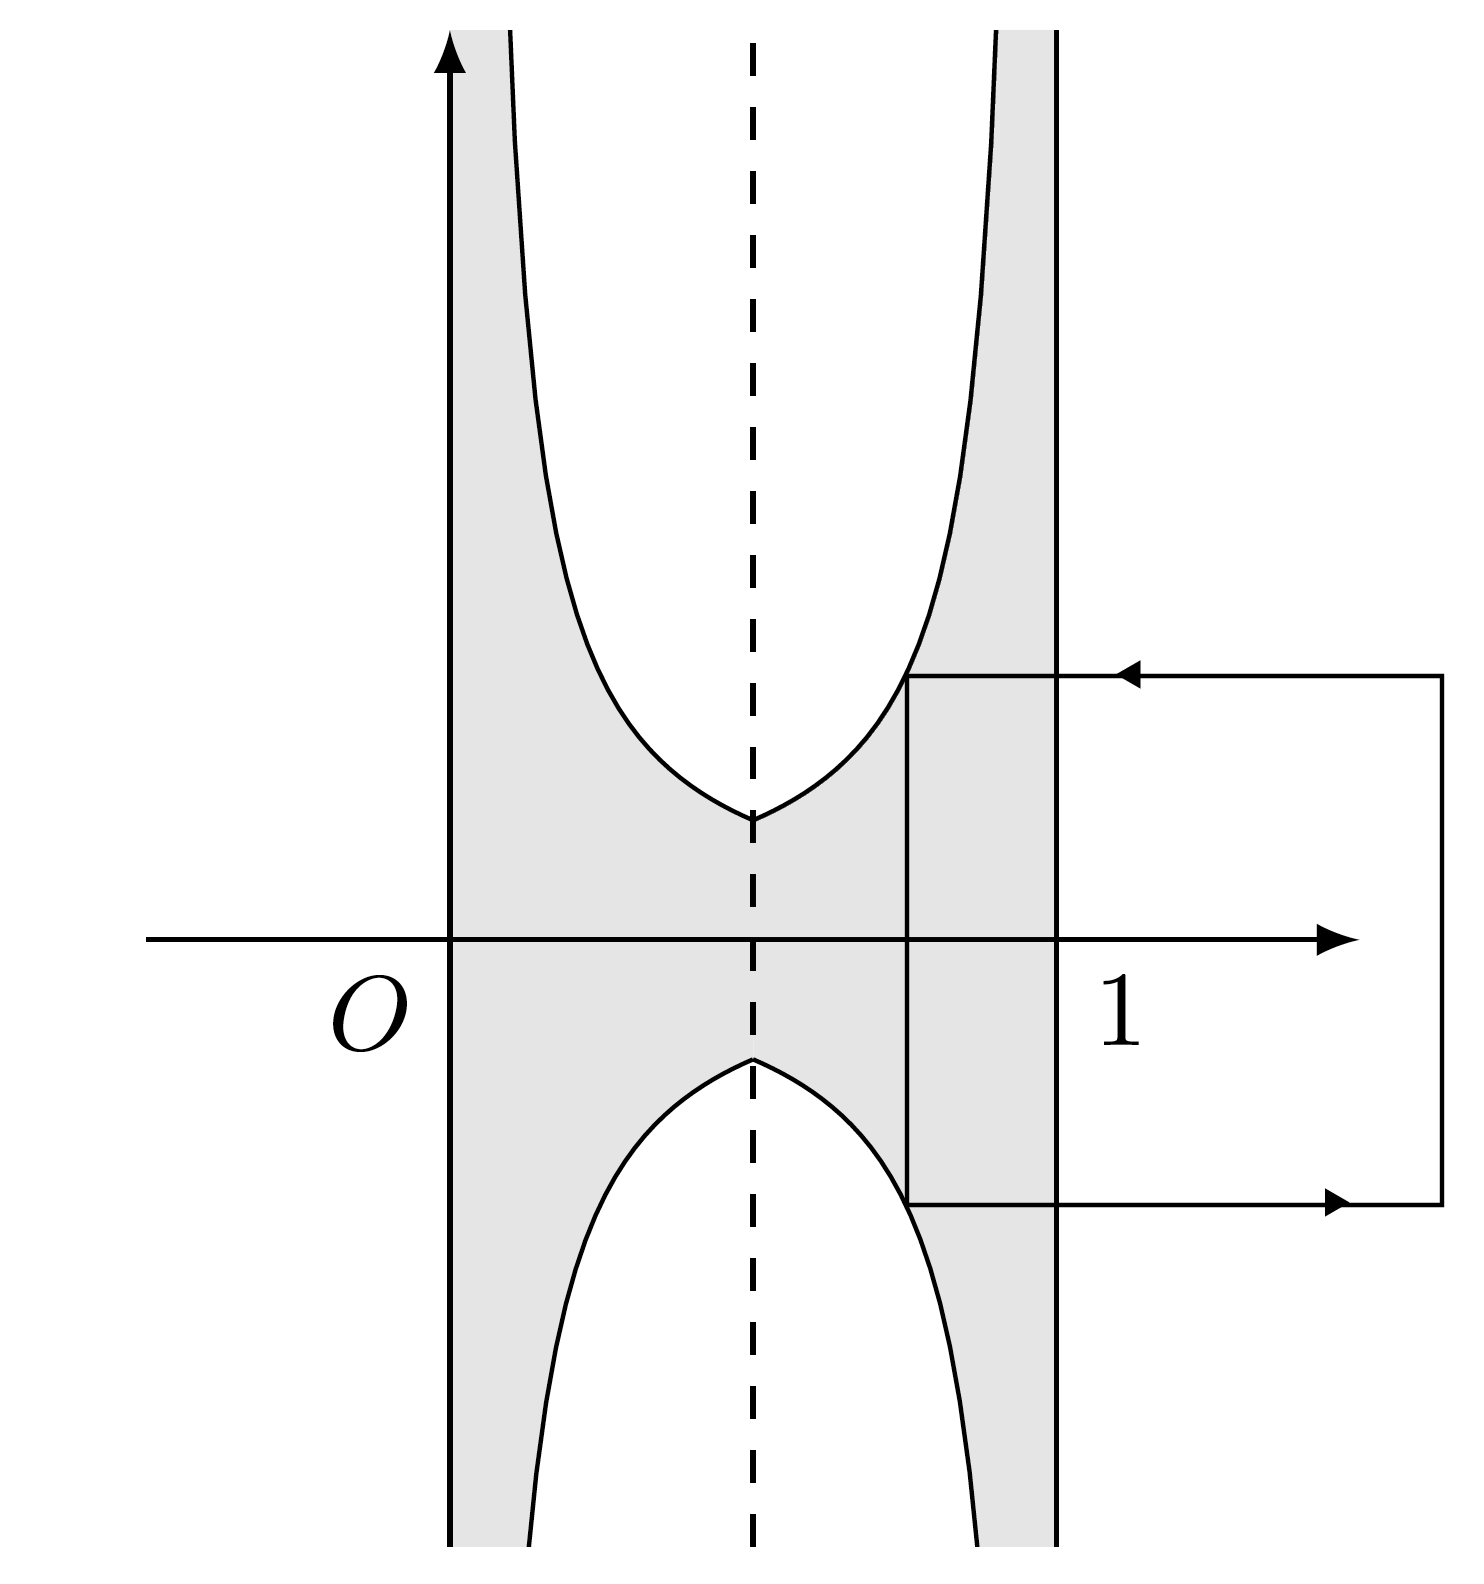
\includegraphics[width=0.8\textwidth]{fig_contour.png}}
      \put(50,50){hello}
      \put(220,60){$\mathbf{R}$}
      \put(150,175){$\sigma_0+iT$}
      \put(150,60){$\sigma_0-iT$}
      \put(255,175){$\sigma_1+iT$}
      \put(255,60){$\sigma_1-iT$}
    \end{picture}
    \label{fig:contour-classique}
  \end{figure}

  On réécrit (voir figure \ref{fig:contour-classique}) :
  \begin{equation}\label{eq:tnp-3-integrales}
    \psi(x) = x +\frac{1}{2\pi i}\left(
      \int_{\sigma_0-iT}^{\sigma_0+iT}
      +\int_{\sigma_0+iT}^{\sigma_1+iT}
      -\int_{\sigma_0-iT}^{\sigma_1-iT}
    \right)
    +O\left(\frac{x\ln^2x}{T}\right)
  \end{equation}
  Mais cette fois, sur les deux segments horizontaux $I_h$ et $I_b$ qui sont $[\sigma_0\pm iT,\sigma_1\pm iT]$, on a, utilisant la proposition \ref{prop:majoration-zeta-zeta-prime-region-classique},
  \begin{align}
    |f(s)| = \left|\left(-\frac{\zeta'(s)}{\zeta(s)}\right)\frac{x^s}{s}\right| & \leq\frac{x^{\sigma_1}}{T}\max_{I_h}\left|\frac{\zeta'}{\zeta}\right| \\
    & = O\left(\frac{x^{\sigma_1}\ln(T)}{T}\right) \\
    & = O\left(\frac{x\ln x}{T}\right) \label{eq:tnp-grand-O}
  \end{align}
  où la dernière égalité vient du fait que l'on n'oubliera pas, à la fin de la preuve, de choisir $T$ tel que $T=O(x)$.

  Sur le segment vertical de gauche $I_g=[\sigma_0-iT, \sigma_0+iT]$, on a
  \begin{align*}
    |f(s)| = \left|\left(-\frac{\zeta'(s)}{\zeta(s)}\right)\frac{x^s}{s}\right| & \leq\frac{x^{\sigma_0}}{|s|}\max_{I_g}\left|\frac{\zeta'}{\zeta}\right| \\
    & = O\left(\frac{x^{\sigma_0}\ln T}{|s|}\right) \\
    & = O\left(\frac{x^{1-c/\ln T}\ln x}{|s|}\right)
  \end{align*}
  où la deuxième ligne est justifiée par la proposition \ref{prop:majoration-zeta-zeta-prime-region-classique}.

  En réassemblant tout, on obtient
  \begin{align*}
    \psi(x) &= x + O\left(x^{1-\frac{c}{\ln T}}\ln x\int_{-T}^T\frac{\mathrm{d}t}{1+|t|}\right) + O\left(\frac{x\ln^2x}{T}\right) \\
    &= x + O\left(x\ln^2 x\left(\mathrm{e}^{-\frac{c\ln x}{\ln T}}+\mathrm{e}^{-\ln T}\right)\right)
  \end{align*}

  En choisissant alors $T:=\mathrm{e}^{\sqrt{c\ln x}}$, on vérifie que $T=O(x)$ pour que \ref{eq:tnp-grand-O} soit justifiée, et on a aussi dans ce cas
  \[ \psi(x)=x+O(x\mathrm{e}^{-c\sqrt{\ln x}}) \]
\end{proof}

%%%%%%%%%%%%%%%%%%%%%%%%%%%%%%%%%%%%%%%%%%%%%%%%%%%%%%%%%%%%%%%%%%%%%%%%%%%%%%%%
%%%%%%%%%%%%%%%%%%%%%%%%%%%%%%%%%%%%%%%%%%%%%%%%%%%%%%%%%%%%%%%%%%%%%%%%%%%%%%%%
\section{Enoncé avec $\pi(x)$}
%%%%%%%%%%%%%%%%%%%%%%%%%%%%%%%%%%%%%%%%%%%%%%%%%%%%%%%%%%%%%%%%%%%%%%%%%%%%%%%%
%%%%%%%%%%%%%%%%%%%%%%%%%%%%%%%%%%%%%%%%%%%%%%%%%%%%%%%%%%%%%%%%%%%%%%%%%%%%%%%%

Nous avons vu, dans les deux section précédentes, deux théorèmes que nous avons appelés "théorème des nombres premiers", mais qui ne faisaient intervenir que $\psi(x)$, sans aucun lien apparent avec $\pi(x)$. Le théorème des nombres premiers s'appelle ainsi parce qu'il a quelque chose à dire sur la distribution des nombres premiers :

\begin{theorem}[Théorème des nombres premiers]\label{eq:tnp-pi-x}
  Il existe une constante réelle $c>0$ telle que l'on ait, au voisinage de $+\infty$,
  \[ \pi(x) = \mathrm{Li}(x) + O(x\mathrm{e}^{-c\sqrt{\ln x}}). \]
\end{theorem}

On rappelle la définition de $\mathrm{Li}$ :

\begin{definition}[Logarithme intégral] On définit la fonction d'écart logarithmique intégrale :
  \[
    \mathrm{Li}(x)
    = \int_2^x\frac{\mathrm{d}u}{\ln u}
  \]
\end{definition}

et on l'accompagne d'une petite proposition :

\begin{proposition}\label{prop:li-development-asymptotique}
  Au voisinage de $+\infty$,
  \[
    \mathrm{Li}(x)
    \sim \frac{x}{\ln x}
  \]
\end{proposition}

\begin{proof}
  En intégrant le terme 1 et en dérivant le terme $1/\ln u$ dans la définition de $\mathrm{Li}$, on a par intégration par parties :
  \begin{equation}\label{eq:li-ipp}
    \mathrm{Li}(x)=\frac{x}{\ln x}-\frac{2}{\ln2}+\int_2^x\frac{\mathrm{d}u}{\ln^2u}.
  \end{equation}

  Or $u\mapsto 1/\ln^2 u = o(1/\ln u)$, donc la dernière intégrale est négligeable devant $\mathrm{Li}$, d'où le résultat.
\end{proof}

\begin{lemma}\label{lem:psi-x-r}
  Soit $R:\mathbb{R}\to\mathbb{R}$ une fonction intégrable, croissante et strictement positive, telle que l'on ait, au voisinage de $+\infty$ : $\psi(x)=x+O(R(x))$. Alors, au voisinage de $+\infty$ :
  \[
    \pi(x)
    = \mathrm{Li}(x)
    + O\left(\frac{R(x)}{\ln x} + R(\sqrt{x}) + \sqrt{x}\right)
  \]
\end{lemma}

\begin{proof}
  Appliquons la formule d'Abel \ref{lem:formule-abel} avec $f(x)=\frac{1}{\ln x}$ et $A(x)=\pi(x)=\sum_{2\leq n\leq x}a_nf(n)$ où $a_n$ vaut $\ln p$ si $n=p$ est un nombre premier et 0 sinon. On obtient :
  \[
    \pi(x)
    = \frac{\theta(x)}{\ln x}
    + \int_2^x{\frac{\theta(u)}{u\ln^2u}}\mathrm{d}u
  \]

  Or on a vu, dans la proposition \ref{prop:relation-psi-theta}, $\psi(x) = \theta(x)+O(\sqrt{x}\ln x)$, donc en combinant avec l'hypothèse de l'énoncé sur $\psi$, on a $\theta(x) = x + O(R(x)+\sqrt{x}\ln x)$. On remplace alors :
  \begin{align*}
    \pi(x)
    &= \frac{x}{\ln x} \\
    &\quad + O\left(\frac{R(x)}{\ln x} + \sqrt{x}\right) \\
    &\quad + \int_2^x\frac{\mathrm{d}u}{\ln^2 u}
    + \int_2^x\left( O\left(\frac{R(u)}{u\ln^2 u}\right) + O\left(\frac{1}{\sqrt{u}\ln u}\right) \right)\mathrm{d}u. \\
    &= \mathrm{Li}(x) + \frac{2}{\ln2} - \int_2^x{\frac{\mathrm{d}u}{\ln^2 u}}\\
    &\quad + O\left(\frac{R(x)}{\ln x} + \sqrt{x}\right) \\
    &\quad + \int_2^x\frac{\mathrm{d}u}{\ln^2 u}
    + \int_2^x\left( O\left(\frac{R(u)}{u\ln^2 u}\right) + O\left(\frac{1}{\sqrt{u}\ln u}\right) \right)\mathrm{d}u \\
    &= \mathrm{Li}(x) \\
    &\quad + O\left(\frac{R(x)}{\ln x} + \sqrt{x}\right) \\
    &\quad + \int_2^x O\left(\frac{R(u)}{u\ln^2 u}\right)\mathrm{d}u
    + \int_2^xO\left(\frac{1}{\sqrt{u}\ln u}\right)\mathrm{d}u
  \end{align*}

  où, à la ligne 2, on a fait apparaître $\mathrm{Li}$ grâce à l'équation \ref{eq:li-ipp} un peu plus haut; et à la ligne 3, $\frac{2}{\ln2}$ a été absorbé dans $O(\sqrt{x})$ et les deux $\int_2^x\frac{\mathrm{d}u}{\ln^2 u}$ s'annulent.
  \\

  On va maintenant étudier indépendamment les deux intégrales de la dernière ligne.
  \\

  \textbf{1ère intégrale}. Comme on étudie le comportement en $+\infty$, on peut supposer $x\geq4$, et donc on peut découper l'intégrale en 2 parties au point $\sqrt{x}$, et, en utilisant le fait que $R$ est croissante, majorer simplement:
  \begin{align*}
    \int_2^x \frac{R(u)}{u\ln^2 u}\mathrm{d}u
    &\leq R(\sqrt{x})\int_2^{\sqrt{x}} \frac{1}{u\ln^2u}\mathrm{d}u
    + R(x)\int_{\sqrt{x}}^x \frac{1}{u\ln^2u}\mathrm{d}u \\
    &= R(\sqrt{x})\int_2^{\sqrt{x}} \frac{1}{u\ln^2u}\mathrm{d}u
    + R(x)\left(\frac{1}{\ln x}-\frac{2}{\ln x}\right)
  \end{align*}
  
  Or l'intégrale restante est une intégrale de Bertrand convergente, donc :
  \[
    \int_2^x \frac{R(u)}{u\ln^2 u}\mathrm{d}u
    = O(R(\sqrt{x})) + O\left(\frac{R(x)}{\ln x}\right).
  \]
  \\

  \textbf{2nde intégrale}. Posons pour tout $x\geq2$,
  \[
    f(x) = \int_2^x\frac{1}{\sqrt{u}\ln u}\mathrm{d}u - \sqrt{x}.
  \]
  Sa dérivée s'écrit :
  \[
    f'(x)=\frac{2-\ln x}{2\sqrt{x}\ln x}.
  \]

  Donc $f'(x)<0\Leftrightarrow x>\mathrm{e}^2$, avec $f(e^2)\approx-0.72<0$. Donc $f$ est strictement négative, et donc :
  \[
    \int_2^x\frac{1}{\sqrt{u}\ln u}\mathrm{d}u 
    \leq \sqrt{x}
    = O(\sqrt{x}).
  \]

  \textbf{Conclusion}. Il suffit maintenant de remplacer ces deux majorations dans la formule de $\pi(x)$ plus haut.
\end{proof}

\begin{proof}[Démonstration du théorème \ref{eq:tnp-pi-x}]
  Posons, en prenant le $c$ dans le théorème des nombres premiers \ref{thm:tnp-terme-erreur-classique} :
  \[
    R(x) = x\mathrm{e}^{-c\sqrt{\ln x}}.
  \]

  On a
  \[
    R'(x) = \frac{\mathrm{e}^{-c\sqrt{\ln x}}(2\sqrt{\ln x}-c)}{2\sqrt{\ln x}},
  \]

  donc $R$ est positive, strictement croissante pour $x>\mathrm{e}^{c^2/4}$, et intégrable. Le lemme précédent \ref{lem:psi-x-r} donne donc :
  \[
    \pi(x)
    = \mathrm{Li}(x)
    + O\left(\frac{R(x)}{\ln x} + R(\sqrt{x}) + \sqrt{x}\right)
  \]

  On a trivialement $O(\frac{R(x)}{\ln x})=O(R(x))$, $O(R(\sqrt{x}))=O(R(x))$ et $\sqrt{x}=O(R(x))$.
\end{proof}

On en déduit également la forme suivante, plus faible, mais plus répandue :

\begin{theorem}[Théorème des nombres premiers, sans terme d'erreur]\label{eq:tnp-equivalence}
  \[ \pi(x)\sim\mathrm{Li}(x) \]
\end{theorem}

\begin{proof}
  Il suffit juste de voir que le terme d'erreur
  \[
    x\mathrm{e}^{-c\sqrt{\ln x}}
    = o\left(\frac{x}{\ln x}\right)
    = o(\mathrm{Li}(x)).
  \]
\end{proof}

On a donc $\pi(x)\sim\mathrm{Li}(x)\sim\frac{x}{\ln x}$, mais $\mathrm{li}$ donne une meilleure approximation, voir figure \ref{fig:pi_li_xlnx}.
\\

\begin{figure}[h]
  \centering
  \caption{En rouge, $\pi$. En bleu, $\mathrm{Li}$. En vert, $x\mapsto\frac{x}{\ln x}$. Source: \url{https://fr.wikipedia.org}.}
  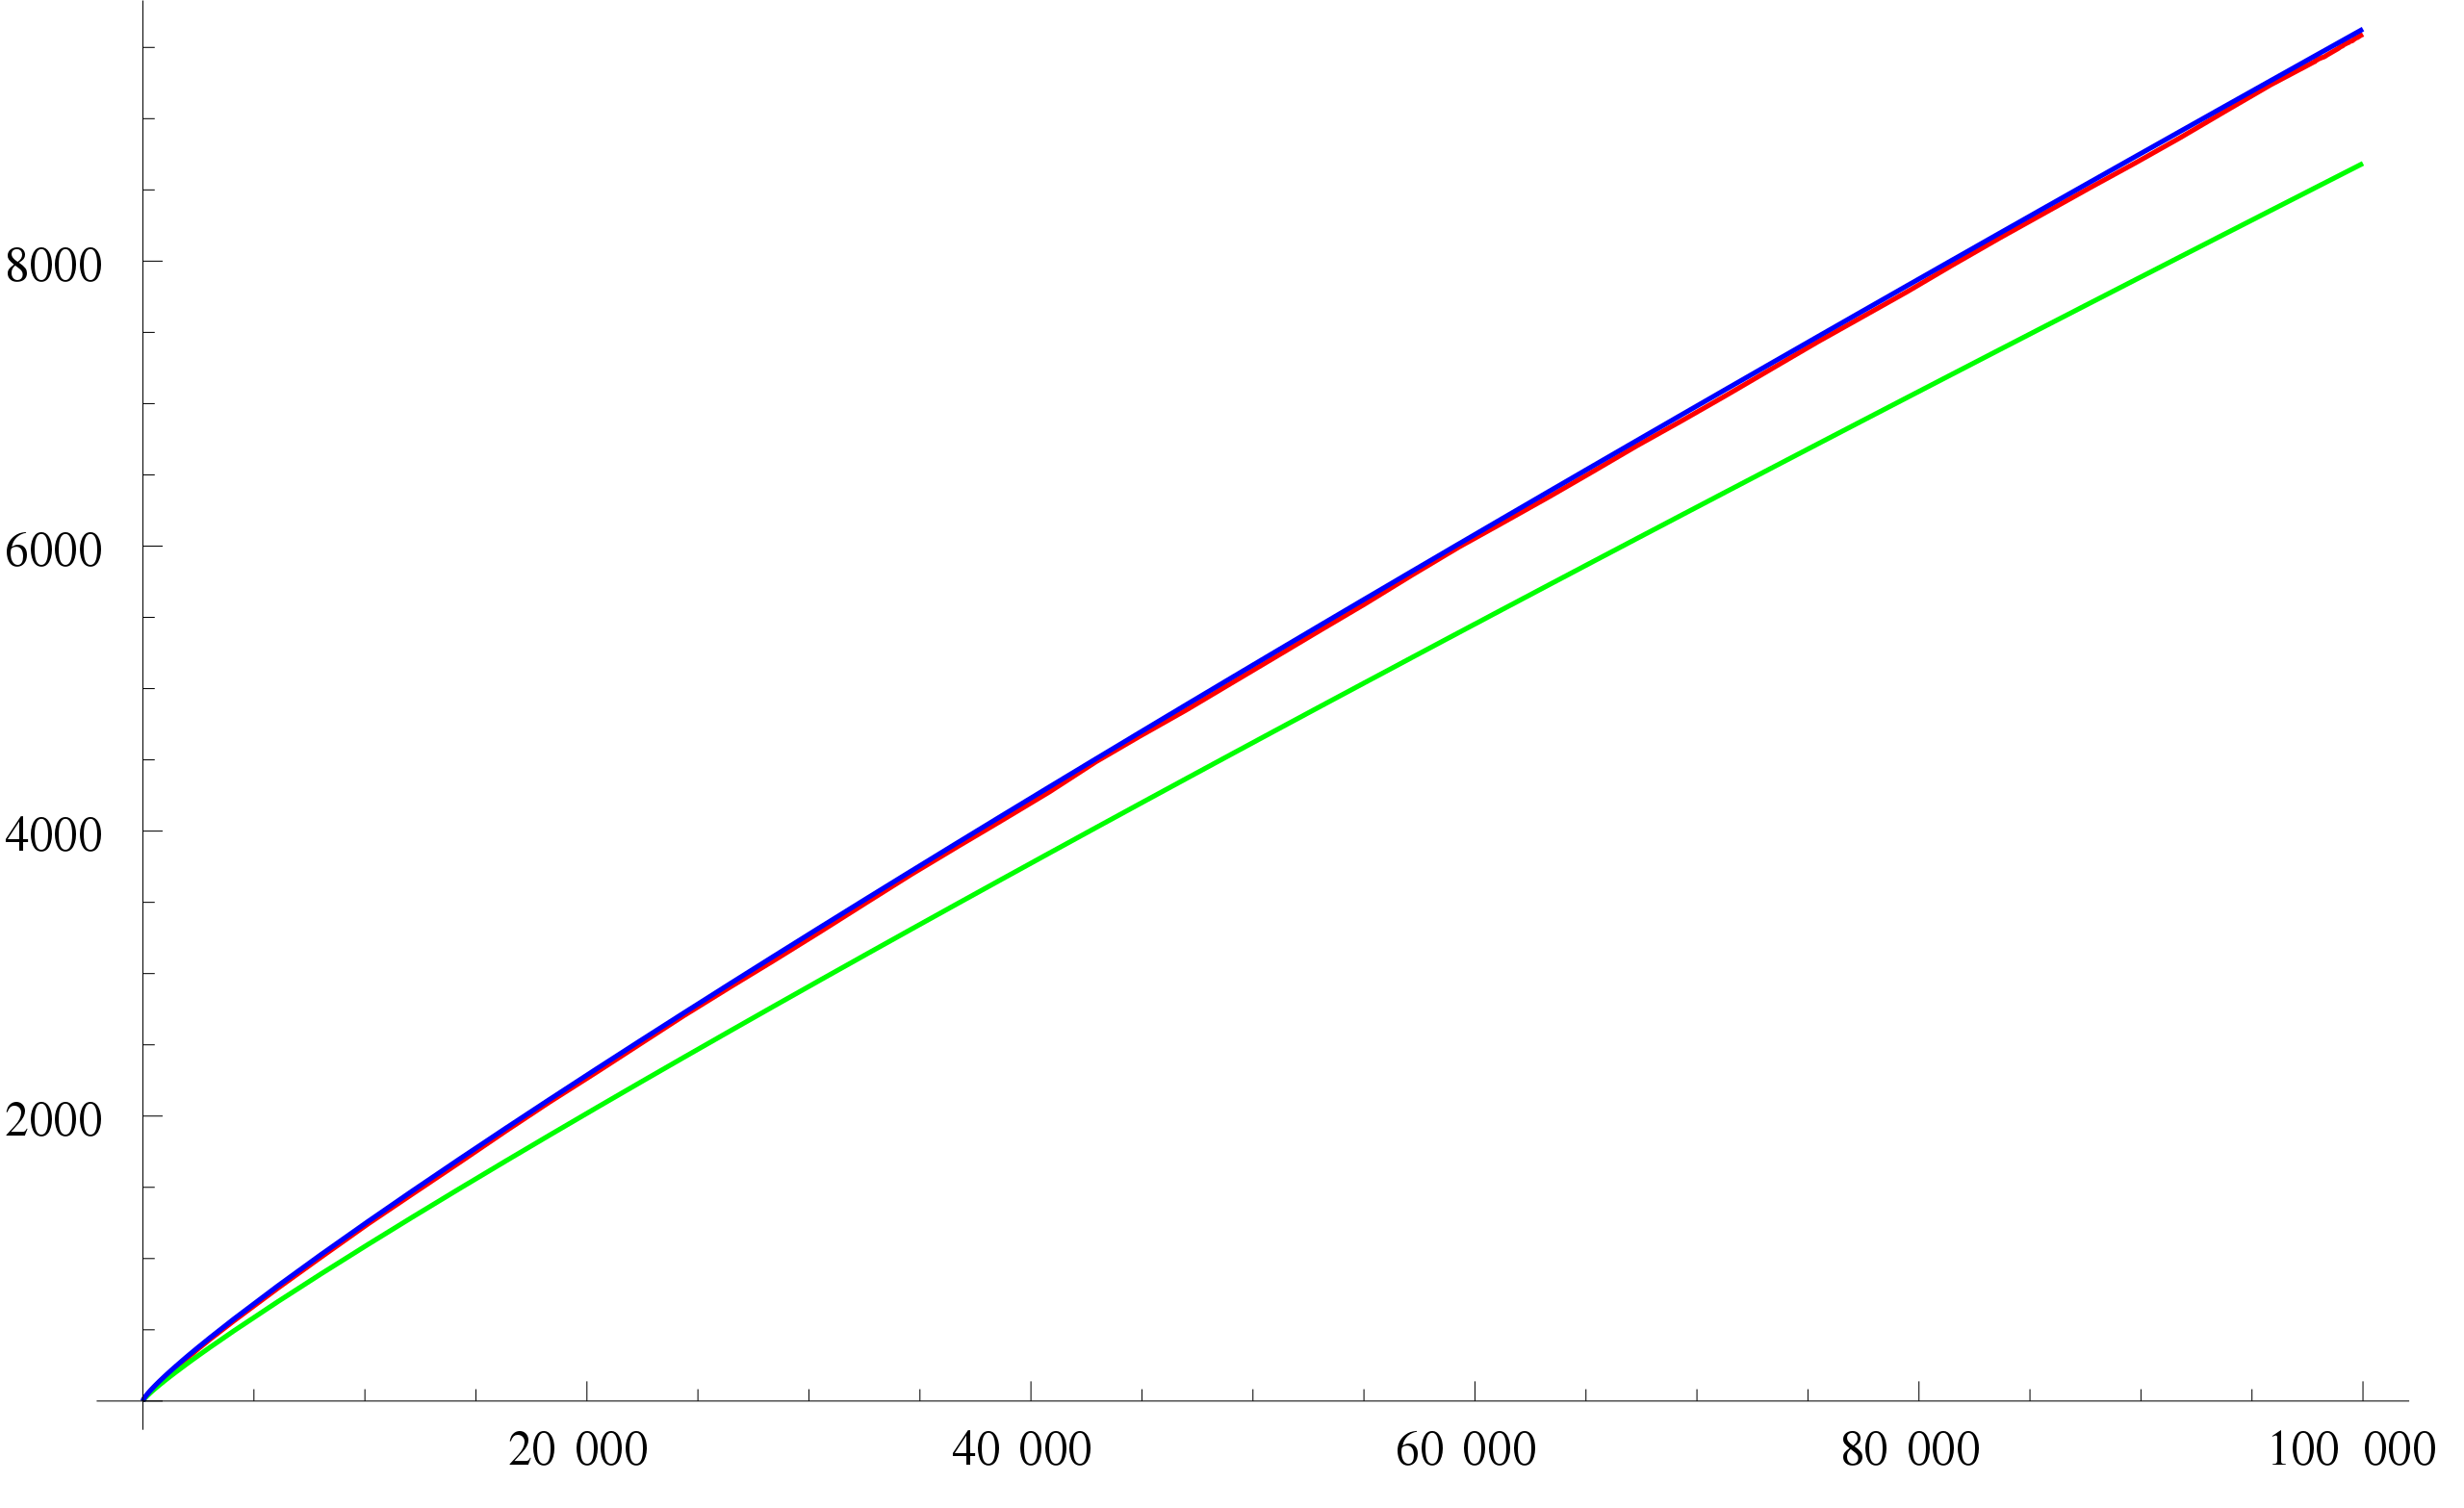
\includegraphics[width=\textwidth]{fig_pi_li_xlnx.png}
  \label{fig:pi_li_xlnx}
\end{figure}

Nous avons donc démontré le théorème des nombres premiers avec terme d'erreur, ce qui permet de clôturer cet exposé.

% %%%%%%%%%%%%%%%%%%%%%%%%%%%%%%%%%%%%%%%%%%%%%%%%%%%%%%%%%%%%%%%%%%%%%%%%%%%%%%%%
% %%%%%%%%%%%%%%%%%%%%%%%%%%%%%%%%%%%%%%%%%%%%%%%%%%%%%%%%%%%%%%%%%%%%%%%%%%%%%%%%
% \section{L'hypothèse de Riemann}
% %%%%%%%%%%%%%%%%%%%%%%%%%%%%%%%%%%%%%%%%%%%%%%%%%%%%%%%%%%%%%%%%%%%%%%%%%%%%%%%%
% %%%%%%%%%%%%%%%%%%%%%%%%%%%%%%%%%%%%%%%%%%%%%%%%%%%%%%%%%%%%%%%%%%%%%%%%%%%%%%%%

% TODO

% \begin{theorem}
%   L'hypothèse de Riemann équivaut à
%   \[ \forall\epsilon>0,\quad\psi(x)=x+O_\epsilon(x^{1/2+\epsilon}) \]
% \end{theorem}

% %%%%%%%%%%%%%%%%%%%%%%%%%%%%%%%%%%%%%%%%%%%%%%%%%%%%%%%%%%%%%%%%%%%%%%%%%%%%%%%%
% %%%%%%%%%%%%%%%%%%%%%%%%%%%%%%%%%%%%%%%%%%%%%%%%%%%%%%%%%%%%%%%%%%%%%%%%%%%%%%%%
% \section{Formule explicite pour $\psi$}
% %%%%%%%%%%%%%%%%%%%%%%%%%%%%%%%%%%%%%%%%%%%%%%%%%%%%%%%%%%%%%%%%%%%%%%%%%%%%%%%%
% %%%%%%%%%%%%%%%%%%%%%%%%%%%%%%%%%%%%%%%%%%%%%%%%%%%%%%%%%%%%%%%%%%%%%%%%%%%%%%%%

\nocite{harvard}
\nocite{standord}

\bibliographystyle{IEEEtranN.bst}
\bibliography{main}{}

Notons que le livre le plus utilisé est sans doute \cite{tenenbaum}.
\end{document}
